%%% CLASS SETTING %%%
\documentclass[doc,natbib,12pt]{apa6}
\usepackage{natbib}
\geometry{margin=1in} % one inch margin (if using apa6)
\bibpunct[, ]{(}{)}{,}{a}{}{,} % sets the punctuation of the bibliography entires.

%%% Paper Information %%%
\title{The Logic and Consequences of Uninformed Voting: The Formal Assessment of Low-Information Competence} % set the title of the document
\shorttitle{The Logic and Consequences of Uninformed Voting}
\author{Gento Kato}
\affiliation{University of California, Davis and Waseda University}
% \twoauthors{Author One}{Author Two}
% \twoaffiliations{Institute of Psychology}{Freud's Institute}
\authornote{Gento Kato is a PhD Candidate, Department of Political Science, University of California, Davis, One Shields Avenue, Davis, CA 95616 USA and a Doctoral Student, Graduate School of Political Science, Waseda University, 1-6-1 Nishiwaseda, Shinjuku, Tokyo 169-8050 Japan (gkato@ucdavis.edu)}
\note{Last Update: October 24, 2018}
\abstract{\singlespacing 
	The scholarly debate on voter competence often considers information as a prerequisite for competent decision-making. It is thus assumed that uninformed voters cannot make active decisions, while fully informed citizenry produces the best democratic outcomes. This study assesses these assumptions by constructing a simple voting model, with two groups of voters: informed and uninformed. The analysis revealed that uninformed voters have different motivations to abstain from the election, depending on the electoral context. Specifically, when the voter population has a moderate ideology, high expressive benefit, and low voting cost, uninformed voters abstain independently due to the voting cost from actively delegating electoral decision making to informed voters. Furthermore, the proposed model of endogenous policy-making shows that the high pivotality of uninformed voters can incentivize policymakers to formulate costly but high-quality policies. The results imply that uninformed voting has the potential to improve democratic accountability.
}
%\rightheader{Social Information and Uninformed Voting Behavior}
%\leftheader{Kato}

% Other Packages/Settings
\usepackage{amsfonts, amsmath, amssymb, bm} %Math fonts and symbols
\usepackage[format=hang, justification=centering]{caption}
\usepackage{dcolumn, multirow} % decimal-aligned columns, multi-row cells
\usepackage{graphicx, subfigure, float} % graphics commands
\usepackage[colorlinks="red"]{hyperref}
\usepackage{setspace}% allows toggling of double/single-spacing
\doublespace % set document spacing to double
\usepackage{enumitem}
\setlist[enumerate]{itemsep=0mm}
%\usepackage{verbatim}% defines environment for un-evaluated code
%\usepackage{endnotes}
%\let\footnote=\endnote
%\usepackage{eurosym} % If using EURO currency sign
%\usepackage{authblk}
%\newcolumntype{d}[1]{D{.}{.}{#1}} % defines a decimal-aligned column
\usepackage{tikz}
\usetikzlibrary{calc}
\newcommand{\floatnote}[1]{\vspace{\abovecaptionskip}\caption*{\textbf{Note:} #1}\vspace{-\abovecaptionskip}}

\begin{document}
	%    \nobibliography*
	% \bibliographystyle{apsr}
	\maketitle
	%    \doublespacing
	
	\par Political information has been considered the prerequisite for voters to make decisions actively and consistently and hold political elites accountable under democracy. Uninformed voters are less likely to vote during elections \citep{Dellicarpini1996wham, Lassen2005thef, Gemenis2014voad} and, even when they vote, their uninformed decisions deviate systematically from those of informed voters \citep{Bartels1996unvo, Fowler2014thpo}. Empirical evidence leads to equating a largely uninformed citizenry with a dysfunctional democracy \citep{Somin1998voig}. However, incompetence is often an assumption rather than an explanation of uninformed voting, as empirical studies rarely provide a logical assessment of how and why information relates to voter competence.
	
	\par This article thus analyzes the logic and consequences of uninformed voting to explore the relationship between information and competence. Competence is defined as the voters' ability to actively make decisions and represent their preferences through a democratic process. The results suggest that the assumption of low-information incompetence is not absolute. The implications are twofold. First, abstention is not necessarily evidence that uninformed voters are overwhelmed by the voting cost to passively withdraw from the election as, in specific circumstances, uninformed voters have an incentive to actively abstain from the election and delegate electoral decisions to informed voters. Second, uninformed voters can improve democratic accountability. Unexpectedly, the significant presence of uninformed voters sometimes motivates policymakers to propose a policy that is costlier for policymakers but more beneficial to voters. Both results imply it is misleading to equate political information with voter competence. The logic of uninformed voting can explain abstention as an active decision, consistent with uninformed voters' interests, and can have the positive consequence of increasing the accountability of political elites.
	
	\par The arguments made in this article also represent a significant departure from the conventional practice of assessing the competence of low-information voters. Previous studies often evaluate the ability to emulate the decisions of informed voters to assess voter competence under low-information \citep{Lupia1994shve, Lupia1998thde, Lau2001adan, Boudreau2009clth}. However, this article suggests that the similarity between uninformed and informed voting behaviors does not necessarily correlate with voter competence. In fact, the separate logic between uninformed and informed voting is what enables uninformed voters to contribute to the welfare of both themselves and the society. This implication opens up a new avenue for assessing low-information voter competence by focusing on the consequences of uninformed decision-making logic, and not how similar uninformed decisions can become to informed decisions. 
	
	\par In the following, I construct a simple model of voting with two representative groups of voters: informed and uninformed. Each group is treated as a unitary actor; thus, they make decisions uniformly. The election occurs in a direct democracy setting, where voters approve or reject the new policy proposal that replaces the status quo policy. This policy proposal has two dimensions, \textit{ideology} and \textit{quality}. For ideology, each voter group has a prior preference of liking or disliking the policy proposal. All voters know about their ideology but are uncertain about the ideologies of others. For quality, the increase in policy quality commonly benefits both voter groups. However, only informed voters know the policy quality with certainty, while uninformed voters are uncertain about whether policy quality is high or low. The electoral outcome is determined by the decision of the pivotal voter group, but voters are uncertain about this pivotal group. If either group of voters abstains, the participating group determines the electoral outcome. In addition to the benefit to the policy outcome, voters receive expressive benefit from making the correct vote choice in the election.
	
	\par In the equilibrium election, highly ideological voters (denoted as \textit{ideologues} in the following) always participate, and vote based on ideology. Among non-ideologues, informed voters always participate, and vote based on policy quality. The central focus of the model is the logic of voting for non-ideologue uninformed voters, as their voting logic is significantly different from that of ideologues and non-ideologue informed voters. Non-ideologue uninformed voters are the only ones who may abstain from the election. Additionally, they change their equilibrium behavior depending on the preferences of other voters (i.e., informed voters). Not only the ideology and quality of the policy proposal but also how informed voters are expected to vote in the election matter in the calculus of uninformed voting.
	
	\par The central results of the baseline model (Proposition 1) identify three occasions where non-ideologue uninformed voters have an incentive to abstain from the election: \textit{discouraged}, \textit{delegatory}, and mixed. 
	Discouraged abstention occurs when uninformed voters fail to overcome the cost of voting due to a combination of uncertainty in policy quality, low efficacy (i.e., the low likelihood of being pivotal in the election), and low expressive benefit. The logic is consistent with the conventional rational choice theory of voting participation \citep{Downs1957anec, Riker1968thof, Matsusaka1995exvo}. Delegatory abstention occurs when uninformed voters benefit from informed voters monopolizing the electoral decision. Independent of the voting cost, uninformed voters are better off abstaining strategically to ensure that informed voters determine the electoral outcome than participating and making uncertain vote choices (Proposition 2). This logic follows the implications of \cite{Feddersen1996thsw, Feddersen1999abin}, but under a vastly simplified, less cognitively demanding setting. Mixed abstention occurs when both discouraged and delegatory abstention incentives are present. The model proposed contributes to the literature by identifying contexts that differentiate the three types of abstention. Additionally, further inquiry reveals that delegatory abstention is the only abstention form that always improves the policy welfare of non-ideologue voters (Proposition 3).
	
	\par In the extension of the baseline voting model, a third actor---the policymaker---endogenously proposes the policy to be voted in the election. In response to voter expected characteristics, he/she proposes either a high or low-quality policy. This setting is similar to the formal models of electoral accountability \citep[e.g.,][]{Prato2016thvo, Prato2018raig}.\footnote{The proposes model does not incorporate the strategic communication between the policymaker and voters. As such, the policymaker has no opportunity to misrepresent himself/herself in the election. Informed voters always learn the policy quality correctly, while uninformed voters never receive information regarding policy quality before they vote.} The policymaker varies in its capacity to formulate policy \citep{Gailmard2007slan, Huber2004buca}: the high-capacity type pays a lower cost to formulate a high-quality policy than the low-capacity type. Further, voters are uncertain about the type of the policymaker. The election occurs in the same setting as the baseline model. 
	
	\par The central focus of the extended model is the decision of the policymaker. A low-capacity policymaker always prefers a low-quality policy, but the high-capacity policymaker may have an incentive to propose a high-quality policy with positive probability. The main results (Propositions 4 and 5) show the existence of a condition where the likelihood of the high-quality policy being proposed is increasing in the pivot probability of uninformed voters. In certain situations, uninformed voters improve, rather than reduce, the accountability of the policymaker. When this improvement occurs, a high-quality policy is more likely under the context of delegatory abstention than under that of discouraged abstention (Proposition 6). The final result (Proposition 7) shows that the increase in accountability does correspond with the increase in voter welfare. The findings imply that the partially uninformed voter group sometimes produces the better democratic outcome.
	
	\par The inquiry in this article adds to the studies on voting behavior and has significant implications regarding the danger of equating low-information with incompetence. First, the analysis deepens the understanding of the decision-making process of uninformed voters. Previous empirical studies often assume that uninformed voter groups have an inactive and inconsistent nature, but this study offers the image of uninformed voters as active and consistent decision makers. Second, the findings provide a new perspective for assessing vote competence. That is, instead of asking if voters are informed enough or how information improves judgment, we should ask how the behavioral rules of uninformed voters affect individual/social welfare. Uninformed voters may not undermine, and can even improve, the quality of the democratic outcome.
	
	\par This article also addresses a broader point on the need to assess the role of electoral context. While we can define informed decisions independently from the electoral environment and outcome, we cannot evaluate decision competence without understanding the environment and the outcome of the election. In specific contexts, the informed decision is not effective or can even be harmful to the competence of voters. Future studies should thus explore contextual factors that affect the relationship between informed and competent decisions.
	
	\section{Conceptualizing Voter Competence}
	
	\par Whether voters can make competent political decisions is one of the most frequently asked questions in the research field of political behavior. In relevant studies, the concept of ``voter competence'' is often discussed in light of how much voters know about politics and their political preference \citep{Converse1964thna, Dellicarpini1996wham, Goren2012onvo}. Such studies treat individuals with informed preference as competent voters and assess how prevalent these voters are in the society. While this approach is intuitive, it excluded the logical relationship between information and competence. That is, it does not explain why and how informed voters help improve the quality of democracy. 
	
	\par This article treats competence and information separately as to assess their relationship. While information indicates the ability of voters to observe their true preference, competence means their ability to offer the effective solution that maximizes their welfare through elections. Competence can be said to have at least two dimensions. 
	First, competence relates to the ability of voters to offer an effective solution to the problem. If uninformed voters have alternative solutions to compensate for lack of information, there is a flaw in the assumption to treat them as less competent than informed voters. Second, competence concerns the welfare of the voter population. If the fully informed public maximizes voter welfare, it can be said that information is an indicator of competence. On the other hand, if a partially uninformed public maximizes voter welfare, information does not necessarily make voters competent.
	
	\par The following analysis shows there exist contexts where uninformed voters choose the effective strategy to substitute information insufficiency, while fully informed voters do not maximize voter welfare. Both findings have an implication that contrasts with the conventional understanding of voter competence. The subsequent paragraphs introduce two existing approaches to evaluating competence and describe how this article provides new insights.
	
	\par The first approach sees information and competence as mutually interchangeable. Given the widely documented concept of ignorance, scholars argue that voters are not competent enough to maintain democracy successfully \citep{Converse1964thna, Dellicarpini1996wham}. Their arguments rely on the evidence that informed and uninformed voters tend to behave differently. These empirical findings suggest that informed electoral participation is increasing political knowledge \citep{Gemenis2014voad, Lassen2005thef}, while informed and uninformed voting patterns differ systematically \citep{Bartels1996unvo, Fowler2014thpo}. The common pessimistic conclusion of this approach among scholars is that the lack of knowledgeable citizens prevents democracy from realizing its ideal. As \cite{Somin1998voig} summarizes, the ``current levels of ignorance strongly suggest that democratic control requires a government far more limited in scope than what we have today'' (446). 
	
	\par The second approach evaluates competence by its similarities with informed decision. This line of research emphasizes the role of information shortcuts \citep{Tversky1974juun} that enable uninformed voters to act as-if informed. Under this approach, scholars argue that the full range of information is unnecessary for uninformed voters to emulate the core preferences and decisions of informed voters \citep{Goren2012onvo, Lupia1998thde, Lupia2016unwh}. However, empirical evidence on the information shortcut approach is mixed. On the positive side, there is evidence that voters do shortcut the information collection process and emulate informed decisions by receiving cues from political endorsement \citep{Lupia1994shve}, public opinion polls \citep{McKelvey1986inel, Sinclair2012frun}, and the media \citep{Popkin1994thre}. Social networks literature also suggests that uninformed voters develop the ability to utilize the political guidance from those who are already effectively informed \citep{Ahn2013exan, Huckfeldt2001thso, Huckfeldt2014nobi}. However, a separate set of empirical studies finds that uninformed voters are not able to utilize information cues effectively. That is, information cues play a weaker role among less informed voters \citep{Hobolt2007tacu, Lau2001adan} and can even bias 
	uninformed decisions away from informed preference \citep{Boudreau2015loin}. As such, there is no final consensus regarding whether information cues are sufficient for voters to act as-if informed. 
	
	\par This article does not deny the existing empirical evidence, but aims to provide a new perspective on the problem of voter competence. I argue that it is too early to treat the systematic differences between informed and uninformed voting behaviors as evidence of the uninformed voters being less competent than informed voters. Similarly, the successful emulation of informed decisions does not necessarily imply competence. The following analysis shows that informed and uninformed voters face separate sets of incentives when making voting decisions. In certain contexts, the fact that informed and uninformed voters behave differently improves, rather than reduces, voter welfare. 
	
	\section{Modeling Uninformed Voting}
	
	\par This article assesses the relationship between information and voter competence by modeling decision-making in elections. The proposed model relaxes two important assumptions set in conventional voting models \citep{Downs1957anec, Riker1968thof}. First, it incorporates information as a variable. The conventional model assumes that all voters possess complete information on their true preference in the election but, apparently, not all voters in the society are informed. Second, the model allows voters to have strategic incentives in voting, while the conventional model assumes voters always make decisions according to individual preferences. In this article, voters make decisions based not only on their preferences but also on the expected decisions of other voters. It is thus natural to assume that individuals care about the decisions of others. 
	
	\par Several existing formal voting studies relax the assumption of informed voters and sincere voting. For instance, \cite{Matsusaka1995exvo} relaxes the first assumption and considers that unformed voters are less certain about their political preferences than informed voters, but his model still assumes voters vote sincerely. On the other hand, \cite{Feddersen1996thsw} construct one of the first voting models that relaxes both assumptions. The equilibrium analysis reveals that uninformed voters have a strategic incentive to abstain, and delegate their votes to informed voters, independent of voting cost. \citeauthor{Feddersen1996thsw} suggest that the ``strategic voting and abstention'' of uninformed voters ``may lead to an informationally superior election outcome'' (418). \cite{Feddersen1999abin} extend the model to the public with heterogeneous preferences and show similar findings regarding rational abstention behavior.
	
	\par The proposed model shares the same motivation as \cite{Feddersen1996thsw, Feddersen1999abin} but in a vastly different setting. First, the proposed model treats voters as groups, not as individuals---informed and uninformed voter groups. The voters within each group share preferences and act uniformly as a group. Typically, the models that deal with the relationship between voters and political elites utilize a similar setting \citep[e.g.,][]{Little2015pran}. In contrast to the voting model with individual voters \citep[i.e.,][]{Feddersen1996thsw, Feddersen1999abin}, this group voting model reduces the number of actors and simplifies the decision calculus. Voters are not expected to make complex calculations of their individual pivotality in the election. Instead, they are expected to make an intuitive conjecture of their group pivotality.
	
	\par Additionally, in the proposed model, voters are uncertain about the distribution of ideology and information in the society, details that are critical in determining the strategic incentives of uninformed voters. In \citeauthor{Feddersen1996thsw}'s model, all voters are assumed to know the exact proportions of ideological and informed voters. However, it is unrealistic to expect (especially for uninformed) voters to know such details about the society. Therefore, my model assumes that voters know the distribution of information and ideology status only with a probability. 
	
	\par The model also consider two critical variables that are not considered by \cite{Feddersen1996thsw, Feddersen1999abin}: the cost of voting and expressive benefit (i.e., the benefit of voting that is not instrumental to the election result). Two variables in the models of \cite{Feddersen1996thsw, Feddersen1999abin} that would allow focus on the role of incentives that are instrumental to the results of the election are omitted. However, as suggested by \cite{Downs1957anec} and \cite{Riker1968thof}, the cost and expressive benefit of voting have been perceived as central to the voting calculus. Without incorporating those two variables, it is difficult to capture a comprehensive picture of the voting process. 
	
	\par Finally, this article goes beyond the incentives of voters and analyzes the relationship between uninformed voting and electoral accountability. Formal studies on politics consider the issue of accountability mainly in two contexts: bureaucratic and executive accountability to the legislative branch \citep[e.g.,][]{Gailmard2013lewh, Patty2017expo} and politicians' accountability to voters in elections \citep[e.g.,][]{Ashworth2012elac, Prato2016thvo}. However, recent evidence from accountability games suggests that fully informative communication between actors in does not necessarily produce the best outcome \citep{Patty2017expo, Prato2016thvo}. It is also argued that seemingly irrational decision of voters is effective in making politicians accountable \citep{Gailmard2018prpr}. This article adds insights to the studies on electoral accountability by analyzing elections with two groups of voters, informed and uninformed. The results are consistent with recent findings: the presence of uninformed voters can produce a better policy outcome than when all voters are informed. 
	
	\section{The Voting Game}
	
	\par This section introduces a referendum voting game, where voters directly vote to approve or reject a single policy proposal. After the election, the status quo policy will be replaced by the proposed policy only if the proposal wins the election.\footnote{Alternatively, the policies can be thought of as candidates in an election, by replacing the status quo policy with the incumbent and the new policy with the challenger.} The quality of the proposed policy is chosen from $q \in \{-1, 1\}$ as follows. If $q=1$, the proposed policy is of high quality and, if $q=-1$, the policy is of low quality.\footnote{The quality of the policy proposal is provided exogenously in the voting game.} The quality of the status quo policy is given as $0$. Therefore, voters gain utility by choosing the high-quality policy proposal ($q=1>0$) and lose utility from the low-quality policy proposal ($q=-1<0$).
	
	\par There are two groups of voters, $g \in \{I, U\}$, both assumed to act as unitary actors. $I$ are informed voters and $U$ are uninformed voters. $I$ know $q$ for sure, while $U$ only know the prior probability of the high-quality policy proposal, $\phi = Pr(q=1) \in [0, 1]$. Separate from information status, each group of voters holds ideology $\beta_g \in \mathbb{R}$, which influences their policy preferences independent of policy quality. Regarding the relationship between information and ideology, informed voters are thought to have stronger and overarching ideologies than uninformed voters \citep{Converse1964thna, Achen2016defo} but recent empirical evidence suggests that, for a specific issue, uninformed voters can have an equally strong ideological preference as informed voters \citep{Broockman2016apto}. Here, the election is assumed to concern one specific policy. Therefore, I follow the recent suggestions and assume that the ideologies of informed and uninformed voters are randomly drawn from the same continuous probability density function $f(\cdot)$.
	
	\par Then, I denote the vote choice as $x_g \in \{0,1\}$ so that $x_g=1$ indicates the vote to accept the policy proposal and $x_g=0$ the vote to reject the policy proposal. The correct vote choice, $r_g$, is captured by the consistency between $x_g$ and voters’ preferences. $r_g$ can be expressed as the function of policy quality $q$ and voters' ideology $\beta_g$:
	\begin{align}
	r_g[q, \beta_g] &= \begin{cases}
	1 &\text{ if } q + \beta_g > 0 \\
	0 &\text{ if } q + \beta_g < 0  \\
	(q + 1)/2 &\text{ if } q + \beta_g = 0\\
	\end{cases}
	\end{align}
	\noindent The above function implies that, if the sum of proposed policy quality and ideology exceeds zero, approving the proposal is the correct choice. If the above sum is negative, rejection is the correct choice.\footnote{If the sum of the proposed quality and ideology is equal to zero, the correct choice is matching the vote with the proposed quality (i.e., accept the policy if and only if the policy is of high-quality).}
	
	\par Additionally, the correct choice function suggests that, on some occasions, voter preferences are determined solely by the ideology. I call those voters \textit{ideologues}. If $\beta_g > 1$, then $r_g[q, \beta_g]$ is always $1$ regardless of $q$ (approval ideologues). Similarly, $\beta_g < -1$ then $r_g[q, \beta_g]$ is always $0$ (rejection ideologues). Remember that $\beta_g$ is randomly drawn from the continuous probability density function $f(\cdot)$. This distribution is common knowledge but the realized value of $\beta_g$ is private information. The probability of ideologues can be represented by the cumulative density function $F(\cdot)$ of $\beta$:
	\begin{align}
	\text{The probability of approval ideologues: } &\kappa_{a} = 1 - Pr(\beta \leq 1) = 1 - F(1)   \\
	\text{The probability of rejection ideologues: } &\kappa_{r} = Pr(\beta \leq -1) = F(-1)   
	\end{align}
	\noindent The remaining type of voters are the \textit{non-ideologues}. Non-ideologue voters may possess ideology, but ideology does not dominate their voting decisions, as they consider both policy quality and ideology to make their decisions. Assume that $1-\kappa_{a} - \kappa_{r} >0$. This condition implies that any voter group can be formed of non-ideologues with positive probability.
	
	\par In addition to the utilities from the electoral outcome, voters gain or lose utility from their actions in the election. This game incorporates two factors discussed in the literature on electoral participation \citep{Downs1957anec, Riker1968thof}. First, it is assumed that voters pay fixed cost $c \in [0,1]$ to participate in the election.\footnote{Think of $c$ as the physical cost of voting, which is expected to be distributed independently from the information status. The main result holds when $c$ differs between voter groups. The cost is assumed not to exceed the utility gain from the high-quality policy being approved (i.e., $c \leq 1$).} If this cost is higher than the expected benefit from participating in the election, voters should choose to abstain from the election. Second, voters receive \textit{expressive benefit} $\varepsilon \in \mathbb{R}^+$ from participating in the election. It is assumed that voters receive expressive benefit when they vote for the option that matches their correct preference (i.e., $x_g=r_g[q, \beta_g]$). This conceptualization of expressive benefit is similar to what is referred to as ``expressive utility'' or ``concern for policy'' in the formal literature \citep{Dewan2008thqu, Kuran1997prtr, Little2015pran}.\footnote{Certain expressive benefit can be given independently of the vote choice. In this game, this \textit{fixed} expressive benefit is incorporated in the cost term, $c$, because it reduces participation cost uniformly.} Additionally, assume $\varepsilon > c$ so that the benefit from expressing the correct preference in voting is always higher than the cost of participating in the election.\footnote{This assumption implies that informed voters always participate in the election and strengthens the finding that uninformed voters have incentives to abstain even with a low or no cost of voting.}
	
	\par Now, I denote the voting participation action of each group of voters as $v_g \in \{0,1\}$ so that $v_g=1$ indicates participation and $v_g=0$ indicates abstention. Additionally, I define the electoral outcome of policy approval as $a=1$ and rejection as $a=0$. The utility functions of voters can be summarized as:
	\begin{align}
	u_g [a,q,\beta_g,v_g,x_g,\varepsilon,c] &= a(\beta_g + q) + v_g(\varepsilon(1-(x_g-r_g[q,\beta_g])^2)-c) \label{uf}
	\end{align}
	
	\par The sequence of the game is as follows. First, according to $\phi = Pr(q=1)$, the new policy is proposed with quality $q$. Second, both voter groups observe their ideology $\beta_g$, but only informed voters $I$ observe the proposed policy quality $q$. In the third step, $I$ and $U$ decide whether to vote for approval, for rejection, or abstain. At the end of the sequence, either $I$ or $U$ is exogenously selected as the pivotal group. $U$ is the pivotal group with probability $\pi \in [0, 1]$ and $I$ with probability $1-\pi$. $\pi$ is common knowledge to all voters. The vote cast by the pivotal group determines the electoral outcome. If the pivotal group abstains, the outcome is determined by the participating voter group. However, if both groups abstain, the policy stays at the status quo.\footnote{This election mechanism is similar to that of the random dictator game \citep{Morton2015whmo}.} In a real-world context, pivot probability $\pi$ is closely on correlation with the population of each voter group. Since the pivotal voter in plurality elections comes from the majority voter group, $\pi$ is equivalent to the likelihood of uninformed voters being the majority group in the society. Voters should also be able to recognize informed and uninformed voters in the society \citep{Huckfeldt2001thso}, but information regarding the exact population of informed and uninformed voters is rarely made available through public media channels (e.g., television, newspapers, radio); it is thus fair to assume that voters have a sense of, but are not certain about, the population of informed and uninformed voters. The pivot probability reflects the incomplete knowledge regarding the majority voter group in the society. Unless $\pi \in \{0, 1\}$, voters are unable to determine the pivot group with certainty.
	
	\section{The Equilibrium Voting Action}
	
	\par This section describes the equilibrium strategies of informed and uninformed voters in the voting game. The decision-making in the voting game is one-shot and involves uncertainty. Therefore, the equilibrium of interest is a Bayesian Nash equilibrium. The equilibrium behavior of ideologue voters (i.e., $\beta_I < -1$ or $\beta_I > 1$) implies the following lemma:
	
	\noindent \textbf{Lemma 1}: \textit{The equilibrium strategy $\{x^*_g, v^*_g\}$ of ideologue voters is to participate in the election and vote in line with their ideology,\footnote{Assume that voters do not play a weakly dominated strategy (i.e., $x_g=1-(q+1)/2$ when $q = - \beta_g$.)}, or} 
	\begin{align}
	x^*_g &= \begin{cases}
	1 &\text{ if } \beta_g > 1 \text{ (approval ideologues)}\\
	0 &\text{ if } \beta_g < -1 \text{ (rejection ideologues)}
	\end{cases} \\
	v^*_g &= 1
	\end{align}
	
	\noindent Then, for non-ideologue voters (i.e., $\beta_g \in [-1, 1]$), the following result holds for those informed: 
	
	\noindent \textbf{Lemma 2}: \textit{The equilibrium strategy $\{x^*_I, v^*_I\}$)of non-ideologue informed voters (i.e., $\beta_I \in [-1, 1]$) is to participate in the election and vote in line with the policy quality, or} 
	\begin{align}
	x^*_I &= (1 + q)/2 \\ 
	v^*_I &= 1
	\end{align}
	
	\par Ideologue voters only need to know the ideology and non-ideologue informed voters only need to know the policy quality to determine their optimal actions. By contrast, non-ideologue uninformed voters face three uncertainties to determine their equilibrium strategy. The first is the uncertainty regarding the quality of the policy proposal ($\phi = Pr(q=1)$), the second is the uncertainty regarding the pivotal group that determines the electoral outcome ($\pi$), and the third is the uncertainty regarding the ideology of informed voters. Informed voters are approval ideologues with probability $\kappa_{a}$, rejection ideologues with probability $\kappa_{r}$, and non-ideologues with probability $1 - \kappa_{a} - \kappa_{r}$. Given the set of beliefs, $\phi$, $\pi$, $\kappa_{a}$, and $\kappa_{r}$, the equilibrium strategy of uninformed voters implies the following lemma:
	
	\noindent \textbf{Lemma 3}: \textit{In the voting game, the equilibrium strategy $\{v^*_U, x^*_U\}$ of non-ideologue uninformed voters (i.e., $\beta_U \in [-1, 1]$) can be represented by a threshold for the expected policy quality ($\phi$), or} 
	\begin{align}
	x^*_U &= 
	\begin{cases}
	1 & \text{if } \phi \geq \phi^*_x = \cfrac{1}{2} - \cfrac{\pi \beta_U}{2(\pi + \varepsilon)}\\
	0 & \text{otherwise}
	\end{cases} \\
	v^*_U &= 
	\begin{cases}
	0 \text{ if } 
	&\phi \geq \phi^*_{v1x0} = min\left\{ \phi^*_x, \phi^*_{vr} = \cfrac{\pi \kappa_{a} (1-\beta_U) + \varepsilon - c}{\pi (\kappa_{a} (1-\beta_U) + (1-\kappa_{r}) (1 + \beta_U))+ \varepsilon} \right\} \\
	&\text{ and } \\ 
	&\phi < \phi^*_{v1x1} =max\left\{ \phi^*_x,  \phi^*_{va} = \cfrac{\pi (1 - \kappa_{a}) (1-\beta_U) + c}{\pi ((1-\kappa_{a}) (1-\beta_U) + \kappa_{r} (1 + \beta_U)) + \varepsilon} \right\} \\
	1 &\text{otherwise}
	\end{cases} 
	\end{align}
	\noindent  $\phi^*_x$ is the \textbf{approval threshold}. Non-ideologue uninformed voters prefer approval over rejection if and only if there exists the probability of a high-quality proposal reaching the approval threshold or higher values. The higher the $\phi^*_x$, the higher is the probability of the high-quality proposal $(\phi = Pr(q=1))$ required to make uninformed voters approve it. Two facts are evident from Lemma 3. First, $\phi^*_x$ is weakly decreasing in ideology $\beta_U$. The higher the ideology, the more attractive the new policy proposal becomes to uninformed voters. Second, the larger the value of expressive benefit $\varepsilon$, the weaker the influence of $\beta_U$ on the approval threshold is (i.e., the threshold sticks to 0.5). However, a strong motivation to express the correct choice incentivizes uninformed voters to use the most conservative approval threshold, regardless of ideology, which is 0.5.
	
	\section{The Logic of Uninformed Abstention}
	
	\par This section explores when and why uninformed voters have reason to abstain from the election. Lemmas 1 and 2 show that ideologue and non-ideologue informed voters have no reason to abstain; the only voters to abstain are non-ideologue uninformed voters. From Lemma 3, the interval between $\phi^*_{v1x0}$ and $\phi^*_{v1x1}$ is the \textbf{abstention interval} (i.e., $[\phi^*_{v1x0},  \phi^*_{v1x1})$). That is, non-ideologue uninformed voters have an incentive to abstain from the election when $\phi$ falls between $\phi^*_{v1x0}$ and $\phi^*_{v1x1}$. The wider this interval, the stronger the incentive for non-ideologue uninformed voters to abstain from the election.
	
	\begin{figure}[t!]
		\caption{Approval Threshold $\phi^*_x$ and Abstention Interval $[\phi^*_{v1x0},  \phi^*_{v1x1})$ Explain the Equilibrium Voting Behavior of Non-ideologue Uninformed Voters}
		\label{fig:abint}
		\begin{center}
			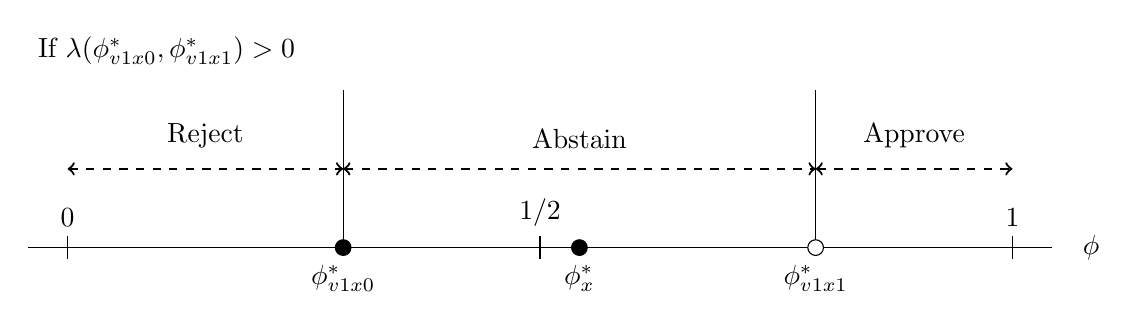
\begin{tikzpicture}
			\tikzstyle{solid node}=[circle,draw,inner sep=2,fill=black];
			\tikzstyle{hollow node}=[circle,draw,inner sep=2, fill=white];
			\draw (-6.5,0)--(6.5,0);
			\foreach \x in {-6,0,6} \draw (\x,0.15)--(\x,-0.15);
			\foreach \x in {-2.5,3.5} \draw (\x,0)--(\x,2);
			\node[above,yshift=4] at (-6,0) {$0$};
			\node[above,yshift=4] at (0,0) {$1/2$};
			\node[above,yshift=4] at (6,0) {$1$};
			\foreach \x in {-2.5,0.5} \node[solid node] at (\x,0) {};
			\foreach \x in {3.5} \node[hollow node] at (\x,0) {};
			\node at (7,0) {$\phi$};
			\node[below,yshift=-3] at (-2.5,0) {$\phi^*_{v1x0}$};
			\node[below,yshift=-3] at (0.5,0) {$\phi^*_{x}$};
			\node[below,yshift=-3] at (3.5,0) {$\phi^*_{v1x1}$};
			\draw[dashed, <->, thick] (-6,1)--(-2.5,1);
			\draw[dashed, <->, thick] (-2.5,1)--(3.5,1);
			\draw[dashed, <->, thick] (3.5,1)--(6,1);
			\node[above,yshift=4] at (-4.25,1) {Reject};
			\node[above,yshift=4] at (0.5,1) {Abstain};
			\node[above,yshift=4] at (4.75,1) {Approve};
			\node[right] at (-6.5,2.5) {If $\lambda(\phi^*_{v1x0},  \phi^*_{v1x1})>0$};            
			\end{tikzpicture}
		\end{center}
		\begin{center}
			\begin{tikzpicture}
			\tikzstyle{solid node}=[circle,draw,inner sep=2,fill=black];
			\tikzstyle{hollow node}=[circle,draw,inner sep=2, fill=white];
			\draw (-6.5,0)--(6.5,0);
			\foreach \x in {-6,0,6} \draw (\x,0.15)--(\x,-0.15);
			\foreach \x in {0.5} \draw (\x,0)--(\x,2);
			\node[above,yshift=4] at (-6,0) {$0$};
			\node[above,yshift=4] at (0,0) {$1/2$};
			\node[above,yshift=4] at (6,0) {$1$};
			\foreach \x in {0.5} \node[solid node] at (\x,0) {};
			\node at (7,0) {$\phi$};
			\node[below,yshift=-3] at (0.5,0) {$\phi^*_{v1x0}=\phi^*_{x}=\phi^*_{v1x1}$};
			\draw[dashed, <->, thick] (-6,1)--(0.5,1);
			\draw[dashed, <->, thick] (0.5,1)--(6,1);
			\node[above,yshift=4] at (-2.75,1) {Reject};
			\node[above,yshift=4] at (3.25,1) {Approve};
			\node[right] at (-6.5,2.5) {If $\lambda(\phi^*_{v1x0},  \phi^*_{v1x1})=0$};            
			\end{tikzpicture}
		\end{center}
		\floatnote{$\beta_U$ is assumed to be the negative value in this figure. $\beta_U=0$ implies that $\phi^*_x=1/2$ and $\beta_U>0$ that $\phi^*_x \leq 1/2$.}
	\end{figure}
	
	\par \autoref{fig:abint} visually illustrates the logic of uninformed abstention. The horizontal axis indicates the prior probability of the high-quality policy ($\phi$), and equilibrium behavior can be represented by the cut-points in $\phi$. I denote the width of the abstention interval as $\lambda(\phi^*_{v1x0},  \phi^*_{v1x1}) = \phi^*_{v1x1} - \phi^*_{v1x0}$. The top panel illustrates abstention behavior when $\lambda(\phi^*_{v1x0},  \phi^*_{v1x1}) > 0$. Under this condition, non-ideologue voters have an incentive to abstain from the election if $\phi$ falls between the lower bound ($\phi^*_{v1x0}$) and upper bound ($\phi^*_{v1x1}$ of the abstention interval. Given that $\phi^*_{v1x0} \leq  \phi^*_x \leq  \phi^*_{v1x1}$, the abstention interval always contains the approval threshold. If $\phi$ is lower than the lower bound (i.e., the low-quality policy is likely), non-ideologue voters participate and vote for rejection. However, if $\phi$ is higher than the upper bound (i.e., the high-quality policy is likely), non-ideologue voters participate and vote for approval. The bottom panel illustrates the voting logic when the width of the abstention interval is zero (i.e., $\lambda(\phi^*_{v1x0},  \phi^*_{v1x1}) =0$). Under this condition, non-ideologue uninformed voters always participate in the election and vote for approval or rejection, depending on the value of the approval threshold. 
	
	\par To understand the movement within the abstention interval, the following general result holds: 
	
	\noindent \textbf{Lemma 4}: \textit{The width of the abstention interval ($\lambda(\phi^*_{v1x0},  \phi^*_{v1x1})$) is weakly increasing in the voting cost ($c$) and weakly decreasing in the expressive benefit ($\varepsilon$), probability of approval ideologues ($\kappa_a$), and probability of rejection ideologues ($\kappa_r$).}
	
	\noindent Lemma 4 shows behavioral patterns consistent with the previous studies on voting. Following this intuition, the voting cost discourages participation, while the expressive benefit encourages participation. Additionally, the motivation for participation is also increasing the likelihood of ideologues. This pattern implies that non-ideologue uninformed voters are motivated to participate in the election when they believe informed voters are highly likely to be ideologues. This implication follows the argument in extant studies that voters with the minority preference tend to have a stronger motivation to participate in the election than those with majority preference \citep{Taylor2010puin, Cantoni2017pras}.
	
	\par In contrast to the above factors, the relationship between the pivot probability of uninformed voters and the abstention interval is conditional. The following proposition describes contexts that transform this relationship:
	
	\noindent \textbf{Proposition 1}: \textit{The lower bound of the abstention interval ($\phi^*_{v1x0}$) is weakly increasing in the uninformed pivot probability ($\pi$) if and only if the probability of ideologues is sufficiently high and the ratio of the expressive benefit to voting cost ($\varepsilon/c$) is sufficiently small, or}
	\begin{align}
	\frac{\kappa_{a} (1 - \beta_U)}{(1-\kappa_{r})(1+\beta_U)} > \varepsilon/c - 1 \label{ecc1}
	\end{align}  
	\noindent \textit{Similarly, the upper bound of the abstention interval ($\phi^*_{v1x1}$) is weakly decreasing in the uninformed pivot probability ($\pi$) if and only if the probability of ideologues is sufficiently high and the ratio of the expressive benefit to voting cost ($\varepsilon/c$) is sufficiently small, or}
	\begin{align}
	\frac{\kappa_{r} (1 + \beta_U)}{(1-\kappa_{a})(1-\beta_U)} > \varepsilon/c - 1 \label{ecc2}
	\end{align}
	
	\noindent Proposition 1 implies there are three possible relationships between the uninformed pivot probability and the abstention interval. \autoref{fig:abgraph} visually depicts the first two relationship forms. Here, the horizontal axis indicates the pivot probability of uninformed voters ($\pi$) and the vertical one the prior probability of the high-quality policy ($\phi$). Non-ideologue uninformed voters have an incentive to abstain from the election when $\phi$ falls within the shaded area. The left-hand panel of the figure shows \textbf{discouraged abstention}: the abstention interval is narrowing in the uninformed pivot probability, both above and below the approval threshold. The right-hand panel of the figure shows \textbf{delegatory abstention}: the abstention interval is widening in the uninformed pivot probability, both above and below the approval threshold. The third type of abstention, \textbf{mixed abstention}, is a combination of the first two forms: the abstention interval is narrowing in $\pi$ for one side of the approval threshold, but widening in $\pi$ for the other side of the threshold.
	
	\begin{figure}[t!]
		\caption{ Visual Depiction of Discouraged and Delegatory Abstention Intervals}
		\label{fig:abgraph}
		\includegraphics[width=\linewidth]{figure/abgraph-1}
		\floatnote{Other parameters are fixed at: $\varepsilon=0.5$, $c=0.3$, and $\beta_U=0$.}
	\end{figure}
	
	\par Discouraged abstention occurs when both inequalities \ref{ecc1} and \ref{ecc2} hold. This condition implies that the lower bound of the abstention interval is increasing and the upper bound is decreasing in $\pi$. This form of abstention is called discouraged since the low probability of being pivotal in election dampens the motivation of non-ideologue uninformed voters to participate in the election. The logic resembles that of the traditional rational choice voting literature \citep{Downs1957anec, Riker1968thof, Matsusaka1995exvo}, in that the combination of low pivot probability, low expressive benefit, and high voting cost leads voters to abstain.
	
	\par Delegatory abstention occurs when neither inequality \ref{ecc1} or \ref{ecc2} hold. This condition implies that the lower bound of the abstention interval is decreasing and the upper bound is increasing in $\pi$. This form of abstention is called delegatory because the logic is similar to that discussed in \cite{Feddersen1996thsw, Feddersen1999abin}. When the probability of being pivotal in the election is high, uninformed voters have the incentive to abstain strategically and \textit{delegate} the electoral outcome to informed voters. In other words, uninformed voters have an incentive to avoid making uncertain vote choices in the election and confuse the electoral outcome. 
	
	\par When only inequality \ref{ecc1} holds, both the lower and upper bounds of the abstention interval are increasing in $\pi$. Similarly, if only inequality \ref{ecc2} holds, both the lower and upper bounds of the abstention interval are decreasing in $\pi$. Those forms of abstention incorporate the logic of both discouraged and delegatory abstention, thus called mixed abstention. Under this condition, discouraged motivation drives abstention for $\phi$ on one side of the approval threshold, while delegatory motivation drives abstention for $\phi$ on the another side.
	
	\begin{figure}[t!]
		\caption{$\varepsilon:c$ Ratio and Probability of Ideologues $\kappa_a$, $\kappa_r$ Explain the Available Form of Abstention}
		\label{fig:abtype}
		\includegraphics[width=\linewidth]{figure/abtype-1}
		\floatnote{$\beta_U$ is fixed at $0$. The absolute values of $\varepsilon$ and $c$ can change, as long as the ratio holds. Additionally, since $\kappa_a + \kappa_r < 1$, the values of $\kappa_a$ and $\kappa_r$ falling within the upper right triangle of each panel do not exist.}
	\end{figure}
	
	\par The likelihood of ideologues ($\kappa_{a}$ and $\kappa_{r}$) and the ratio of the expressive benefit to voting cost ($\varepsilon/c$) play important roles in determining the form of the abstention interval for non-ideologue uninformed voters. \autoref{fig:abtype} summarizes these conditions. The horizontal axis indicates the probability of approval ideologues ($\kappa_a$) and the vertical one the probability of rejection ideologues ($\kappa_r$). The shaded areas represent the form of uninformed abstention possible under the given parameters. The dark (orange) shading indicates that abstention is delegatory, the brighter (green) shading indicates discouraged abstention, and the brightest (yellow) shading indicates mixed abstention. The shaded areas reflect the prevalence of each form of abstention.
	
	\par Each panel of \autoref{fig:abtype} depicts the different ratios of $\varepsilon$ to $c$. Across panels, the area of delegatory abstention is increasing, while the area of discouraged abstention is decreasing as ratio. When $c$ is sufficiently low relative to $\varepsilon$, the only possible abstention type is delegatory (as shown in the rightmost panel). In fact, the following proposition holds for the existence of the abstention interval with a positive width (i.e., $\lambda(\phi^*_{v1x0},\phi^*_{v1x1})>0$):
	
	\noindent \textbf{Proposition 2}: \textit{When $c=0$, discouraged and mixed abstention intervals with $\lambda(\phi^*_{v1x0},\phi^*_{v1x1})>0$ never exist. On the other hand, a delegatory abstention interval with $\lambda(\phi^*_{v1x0},\phi^*_{v1x1})>0$ exists for a sufficiently high $\pi$ and sufficiently low $\kappa_a$, $\kappa_r$, and $\varepsilon$.}
	
	\noindent Proposition 2 follows the implications of \cite{Feddersen1996thsw}, who argue that delegatory abstention occurs independently of the voting cost. Note that the absolute value of $\varepsilon$ must be sufficiently low to ensure the existence of a non-zero delegatory abstention interval. For delegatory abstention to occur, the expressive benefit must be sufficiently high relative to the voting cost but sufficiently low in absolute value. This pattern emerges because a high expressive benefit reduces the relative importance of receiving instrumental utility from policy quality (which is fixed to $-1$ and $1$ in this game). However, if the absolute value of the expressive benefit is too high, uninformed voters are better off voting than abstaining even if the likelihood of the correct choice is low.
	
	\par In the left-hand and central panels of \autoref{fig:abtype} (i.e., voting cost is sufficiently high relative to the expressive benefit), the prior probability of ideologue voters plays an important role in determining what form of abstention may occur. Inequalities \ref{ecc1} and \ref{ecc2} imply that, when voters are non-ideologues for sure (i.e., $\kappa_{a} = \kappa_{r} = 0$), only delegatory abstention is possible. Delegatory motivation leads to abstention when non-ideologue uninformed voters expect informed voters to share the same preference. An increase in the likelihood of ideologues makes discouraged abstention more likely than delegatory abstention. If informed voters are highly likely to be ideologues, non-ideologue uninformed voters lose the incentive to delegate votes. Under this condition, abstention occurs only due to discouragement from the high voting cost. Mixed abstention tends to occur when the likelihoods of approval ideologues and of rejection ideologues differ significantly. If $\kappa_a$ is significantly higher than $\kappa_r$ (the bottom right corner of each panel), delegatory motivation drives abstention when non-ideologue uninformed voters relatively prefer the approval vote (i.e., $\phi \geq \phi^*_x$) and discouraged motivation drives abstention when non-ideologue uninformed voters relatively prefer the rejection vote (i.e., $\phi < \phi^*_x$). The opposite pattern occurs if $\kappa_r$ is significantly higher than $\kappa_a$ (the top left corner of each panel).
	
	\par The above uninformed voting logic unifies the two different explanations of uninformed abstention discussed in the literature. Discouraged abstention follows the classic logic of political participation \citep{Downs1957anec} to see abstention as the product of high voting cost and low electoral efficacy. Delegatory abstention supports the contrasting view suggested by \cite{Feddersen1996thsw} to understand uninformed abstention as the active delegation of the electoral decision to informed voters. Proposition 1 identifies electoral contexts that condition the occurrence of different abstention forms. When the voting cost is sufficiently low and the likelihood of informed voters sharing the same preference as non-ideologue uninformed voters is sufficiently high, the abstention of non-ideologue uninformed voters occurs as a result of active delegation rather than discouraged inactivity.
	
	\par Additionally, the following result can be derived regarding the relationship between the form of abstention and the policy utility instrumental to the electoral outcome:
	
	\noindent \textbf{Proposition 3}: \textit{It is always the case that the expected policy utility of non-ideologue uninformed voters (i.e., $E[a(\beta_U + q)]$) is weakly increasing in delegatory abstention. However, there exists a condition where the expected policy utility of non-ideologue uninformed voters is decreasing in discouraged abstention.}
	
	\noindent Proposition 3 implies that, while discouraged abstention has the potential to reduce instrumental policy utility, delegatory abstention has not. Since abstention occurs only for non-ideologue uninformed voters, this means that delegatory abstention is an effective strategy to increase the likelihood of the high-quality policy being approved and the low-quality policy being rejected. In a context where delegatory abstention is possible, uninformed voters use abstention as an alternative information tool that always increases the likelihood of the preferred electoral outcome.
	
	\section{The Accountability Game}
	
	\par Here, I extend the voting game to consider the situation where the proposed policy quality is endogenously determined by a third actor. I call this new game the accountability game. For simplicity, assume that the ideology is chosen from three discrete categories ($\beta_g \in \{-R, 0, A\}$ where $R>1$ and $A>1$).\footnote{This assumption is a special case of the ideology distribution $f(\cdot)$, and implies that $\beta_U$ for non-ideologue voters is always zero. The discrete distribution is chosen to avoid an overly complicated, counter-intuitive strategic calculation for the policymaker.} This game inherits almost all settings of the voting game but has an additional stage at the beginning: the policymaker $P$ proposes policy proposal $q$.
	
	\par Formal studies on policy-making suggest that a policymaker may have a differential capacity to formulate a high-quality policy \cite[e.g.,][]{Gailmard2007slan, Huber2004buca}. As such, in the accountability game, assume there are two types of policymakers $T \in \{H, L\}$: high-capacity $P_H$ and low-capacity $P_L$. The two types differ in the level of effort required to formulate the policy. The high-capacity policymaker puts relatively low effort $\eta_H = 1$ to achieve the high quality compared to the low-capacity policymaker (who needs $\eta_L = 2$ to achieve the high-quality policy). Further, assume that the policymaker gains a fixed positive benefit ($B=2$) from the new policy being approved in the election.\footnote{The default values normalize the cost of policymaking. The general result holds as long as $\eta_H < B \leq \eta_L$.} One can understand $B$ as the motivation for policymakers to appear effective in creating the policy. Consequently, the utility function of $P$ is defined as:
	\begin{align}
	u_P = \begin{cases}
	2 - \eta_T \cdot \cfrac{1+q}{2} &\text{ if the policy is approved} \\
	- \eta_T \cdot \cfrac{1+q}{2} &\text{ if the policy is rejected} \\
	\end{cases} \label{acuf}
	\end{align}
	\noindent Regardless of the electoral outcome, the policymaker has to put effort $\eta_T$ into formulating the high-quality policy ($q=1$). On the other hand, the low-quality policy can be formulated without this effort. Then, if the policy is approved, the policymaker receives approval benefit $B=2$. 
	
	\par The utility function represented in \autoref{acuf} implies the following lemma regarding the equilibrium decision of the low-capacity policymaker:
	
	\noindent \textbf{Lemma 5}: \textit{The equilibrium strategy of the low-capacity policymaker $P_L$ is to always propose the low-quality policy ($q=-1$).}
	
	\noindent Lemma 5 shows that the low-capacity policymaker always proposes the low-quality policy ($q=-1$) at equilibrium. The approval benefit ($B=2$) fails to make up for the effort level required for the high-quality policy ($\eta_L=2$). Therefore, only the high-capacity policymaker is potentially responsive to expected voting behavior in the election. 
	
	\par The type of policymaker is not common knowledge, and all voters form belief $p \in [0, 1]$, which indicates the probability of the high-capacity policymaker. Since the low-capacity policymaker always proposes the low-quality policy (Lemma 5), voters are only uncertain about the decisions of the high-capacity policymaker. I denote $\phi_H \in [0,1]$ as the probability that the high-capacity policymaker formulates a high-quality policy (i.e., the mixed strategy of the high-capacity policymaker). Given that only the high-capacity policymaker can potentially formulate the high-quality policy, voters' prior belief regarding the probability of high-policy quality is represented by $\phi = p \cdot \phi_H$.
	
	\par The sequence of the accountability game is as follows. First, nature selects the high-capacity policymaker with probability $p$ and the low-capacity policymaker with $1-p$. Then, the selected policymaker ($P_T$) decides whether to propose the high- or low-quality policy by $\phi_T = Pr(q=1) \in [0, 1]$. Only informed voters observe the quality of the policy with certainty. If $\phi_T = 0$, the policymaker of type $T$ proposes the low-quality policy for sure; if $\phi_T = 1$, the policymaker of type $T$ proposes the high-quality policy for sure. The election in the accountability game is conducted identically to the voting game. 
	
	\par Since the accountability game also involves the dynamic process of decision-making, the appropriate equilibrium of interest is a perfect Bayesian equilibrium. The analytical result of the voting game (Lemmas 1--3) still explains the equilibrium behavioral rule of voters because the two games share the same voting process. The focus of this section is describing the behavior of the policymaker. To establish the baseline behavior, assume that informed voters are always pivotal in determining the electoral outcome ($\pi=0$). The following proposition reflects the equilibrium behavior of the high-capacity policymaker:
	
	\noindent \textbf{Proposition 4}: \textit{Assume that $\pi=0$. $P_H$ proposes the high-quality policy for sure if the probability of ideologue voters is sufficiently high and the low-quality policy for sure otherwise, or}
	\begin{align}
	\phi^*_H[\pi=0] &=
	\begin{cases}
	1 &\text{ if }  \kappa_{a} + \kappa_{r} \geq 0.5 \\
	0 &\text{ if }  \kappa_{a} + \kappa_{r} < 0.5
	\end{cases}
	\end{align}
	
	\noindent Proposition 4 provides the starting point of the analysis when informed voters determine the electoral outcome for certain. This condition is equivalent to a fully informed public because all voters who are potentially pivotal in the election are informed. As shown in Lemma 5, the low-capacity policymaker chooses the low-quality policy regardless of the expected actions of the voters. However, if the policymaker is of high capacity, the policy quality decision is solely determined by the likelihood of ideologues. The policymaker proposes the high-quality policy if and only if the combined likelihood of voters being ideologues (i.e., both approval and rejection ideologues) is below $0.5$. The increasing presence of ideologue voters reduces the motivation for a high-quality proposal because policy quality is irrelevant to the decision calculus of ideologue voters (Lemma 1). The policymaker thus prefers the low-quality policy since policy quality is not useful in receiving the approval vote from ideologue voters.
	
	\par On the other hand, the presence of potentially pivotal uninformed voters ($\pi>0$) changes the strategic motivation of the high-capacity policymaker. The following proposition describes patterns of change in the equilibrium decision:
	
	\noindent \textbf{Proposition 5}: \textit{Assume that a change from a fully informed public (i.e., $\pi=0$) to the presence of potentially pivotal uninformed voters (i.e., $\pi>0$) occurs. If the probability of ideologues is below $0.5$ (i.e., $\kappa_{a} + \kappa_{r} < 0.5$), $\phi^*_H$ is weakly decreasing in the change. By contrast, if the probability of ideologues is $0.5$ or above (i.e., $\kappa_{a} + \kappa_{r} \geq 0.5$), $\phi^*_H$ is strictly increasing in the change for a sufficiently high pivot probability of uninformed voters ($\pi$) and prior probability of the high-capacity policymaker ($p$) and sufficiently low probability of ideologues ($\kappa_{a}+\kappa_{r}$).}
	
	\noindent From Proposition 5, two forms of change can occur between the state of fully informed pivotal voters ($\pi=0$) and that of potentially uninformed pivotal voters ($\pi>0$). When the likelihood of ideologues is below that of chance (i.e., $\kappa_{a} + \kappa_{r} < 0.5$), the high-capacity policymaker proposes the high-quality policy ($\phi^*_H=1$) to a fully informed public ($\pi=1$). Under this condition, the positive pivot probability of uninformed voters ($\pi > 0$) may lead to a decrease in $\phi^*_H$. For some positive $\pi$, the equilibrium policy decision moves away from $1$. This form of change is consistent with the existing arguments that information (or informed decision) is crucial for voters to become competent. 
	
	\par A striking contrast can be seen in the form of change under the likelihood of ideologues higher than that of chance (i.e., $\kappa_{a} + \kappa_{r} \geq 0.5$). Under this condition, the high-capacity policymaker always proposes the low-quality policy ($\phi^*_H=0$) to a fully informed public ($\pi=0$). Then, interestingly, the increase in the pivot probability of uninformed voters can lead to an increase in $\phi^*_H$ from $0$ to $\phi^*_{v1x0}/p$ or $\phi^*_{v1x1}/p$. This pattern occurs because the increase in $\phi^*_H$ can improve the policy approval likelihood. By setting $\phi^*_H=\phi^*_{v1x0}/p$, the policymaker can ensure that the non-ideologue uninformed voters abstain from the election (instead of voting for rejection) and by setting $\phi^*_H=\phi^*_{v1x1}/p$ the policymaker can incentivize non-ideologue uninformed voters to vote for approval.
	
	\par The second form of change implies that uninformed voting can have positive consequences. That is, the presence of potentially pivotal uninformed voters can increase the likelihood of high-quality policymaking. When facing a likely-to-be ideological informed public, the high-capacity policymaker loses motivation to formulate the high-quality policy. However, the equally ideological voter population with potentially pivotal uninformed voters may generate an incentive for high-quality policymaking by introducing uncertainty to the electoral outcome. The high-capacity policymaker may thus have an incentive to set the high-quality policy with positive probability so that he/she can prevent non-ideologue uninformed voters from voting for rejection. 
	
	\par When $P_H$ has an incentive to deviate from the low-quality policy ($\phi^*_H=0$), the electoral context determines the choice between $\phi^*_{v1x0}/p$ and $\phi^*_{v1x1}/p$. The following proposition holds for the relationship between the electoral context and the equilibrium policy decision:
	
	\noindent \textbf{Proposition 6}: \textit{Assume that $P_H$ deviates from $\phi^*_H=0$ under $\kappa_a+\kappa_r\geq0.5$. Holding other factors constant, the choice of $\phi^*_{v1x0}/p$ tends to occur under the discouraged abstention context (i.e., low $\varepsilon:c$ ratio) and the choice of $\phi^*_{v1x1}/p$ under the delegatory abstention context (i.e., high $\varepsilon:c$ ratio).}
	
	\noindent Proposition 6 implies that the presence of potentially pivotal uninformed voters can improve policy accountability even more if the electoral context allows them to abstain due to the delegatory than the discouraged motivation. In the delegatory abstention context, $P_H$ tends to be motivated to propose the high-quality policy with high probability to ensure non-ideologue uninformed voters vote for approval. However, in the discouraged abstention context, $P_H$ tends to be better off at suppressing the participation of non-ideologue uninformed voters by proposing the high-quality policy with low probability rather than encouraging them to cast an approval vote.
	
	\begin{figure}[t!]
		\caption{For a Sufficiently High $\pi$, $P_H$ Proposes the Higher-Quality Policy in the Delegatory Abstention Context Rather than the Discouraged Abstention Context}
		\label{fig:eupgraph}
		\includegraphics[width=\linewidth]{figure/eupgraph-1}
		\floatnote{Relevant parameters are fixed to: $\kappa_a = \kappa_r = 0.3$ and $p=0.85$. If $\phi_H$ falls within the shaded interval, non-ideologue uninformed voters abstain from the election.}
	\end{figure}
	
	\par \autoref{fig:eupgraph} illustrates the relationship between the decision calculus of $P_H$ and the presence of potentially pivotal uninformed voters when $\kappa_{r}+\kappa_{a}\geq 0.5$. In each panel, the horizontal axis shows the policy quality decisions of the high-capacity policymaker ($\phi_H \in [0,1]$) and the vertical axis the corresponding expected utilities ($Eu(P_H)$). The equilibrium quality decision ($\phi^*_H$) is determined by the value of $\phi_H$ that maximizes expected utility. The figure focuses on the role of $\pi$ and the form of abstention in changing the equilibrium decision (other parameters are fixed at $\kappa_{r}=\kappa_{a}=0.3$ and $p=0.85$). The shaded area represents the values of $\phi_H$ that motivate non-ideologue uninformed voters to abstain from the election (i.e., corresponds to the interval illustrated in \autoref{fig:abint}). They cast a rejection vote for $\phi_H$ at the left-hand side of the interval and approval vote for $\phi_H$ at the right-hand side of the interval.
	
	\par In each row, the left panel shows $Eu(P_H)$ is strictly decreasing in the probability of high-quality policy proposal by $P_H$ ($\phi_H$). The high-capacity policymaker facing a likely-to-be ideological informed public ($\pi=0$) has no incentive to deviate from the low-quality policy, regardless of the equilibrium decision of non-ideologue uninformed voters. The central panel indicates that, if uninformed voters are potentially pivotal ($\pi>0$), $Eu(P_H)$ is increasing in $\phi_H$ at the cut-points that correspond to the change in uninformed voting behavior. If $\pi$ is sufficiently high (the right-hand panel), expected utility of $P_H$ is maximized at $\phi^*_H>0$.
	
	\par The top row of the figure illustrates the decision calculus when the available form of abstention is discouraged (i.e., high $\varepsilon:c$ ratio, $\varepsilon=0.5$ and $c=0.4$). In this case, the reduction in the abstention interval causes a more substantial increase in the $Eu(P_H)$ at the cut-point corresponding to the lower bound of the abstention interval (i.e., $\phi^*_{v1x0}$) than at the cut-point corresponding to the upper bound. The bottom row shows the opposite case. Under the electoral context with the delegatory abstention (i.e., high $\varepsilon:c$ ratio, $\varepsilon=0.5$ and $c=0.2$), the expansion of the abstention interval causes a more significant increase in $Eu(P_H)$ at the upper bound of the interval than at the lower bound. Consequently, for a sufficiently high $\pi$, $P_H$ proposes the high-quality policy with the higher probability if the available form of abstention is delegatory instead of discouraged.
	
	\par Note that the prior probability of the high-capacity policymaker ($p$) plays a role in the decision calculus of $P_H$. The increase from $\phi^*_H=0$ occurs only when $p$ is sufficiently high. The logic behind this fact is as follows. First, the high-capacity policymaker proposes the high-quality policy with a positive probability only when this action can prevent uninformed voters from voting for rejection. Second, uninformed voters stop voting for rejection only when the prior belief of the high-quality policy proposal (i.e., $\phi = p \cdot \phi_H$) is sufficiently high. Since the low-capacity policymaker never proposes the high-quality policy, a low $p$ dampens the probability of the high-quality policy in general. When $p$ is low (i.e., $p < \phi^*_{v1x0}$), no possible value of $\phi_H$ can convince non-ideologue uninformed voters to stop voting for rejection; thus, $P_H$ sticks to the low-quality policy.
	
	\par The analysis in this section shows that uninformed voting has the potential to improve policy accountability. When the policymaker expects voters to be sufficiently ideological (i.e., $\kappa_{r}+\kappa_{a}\geq0.5$), he/she proposes the low-quality policy at no cost if all pivotal voters are fully informed; however, he/she may pay the cost to formulate the high-quality policy if uninformed voters are potentially pivotal. Furthermore, if the policymaker proposes the high-quality policy with positive probability, this probability tends to be higher in electoral contexts where the available form of uninformed abstention is delegatory rather than discouraged.
	
	\section{Non-Ideologue Voter Welfare}
	
	\par The previous section showed that policy accountability can increase in response to uninformed voting. This section extends the analysis to consider its implications on voter welfare. Since ideologue voters do not care about the quality of the policy, I focus on non-ideologue voters to determine if the presence of potentially uninformed pivotal voters can improve welfare.\footnote{The same result holds for the entire voter population, as long as the ideology distribution of the society is ``balanced'' (i.e., $\kappa_r R = \kappa_a A$).} To calculate the welfare of the voter population, I define $\psi$ as the proportion of uninformed voters and $1-\psi$ as that of informed voters. Assume that $\psi$ is randomly drawn from the continuous probability density function $\gamma(\cdot)$ defined on the interval $[0, 1]$ and 
	only $\gamma(\cdot)$ is common knowledge. Then, it is obvious that the uninformed pivot probability ($\pi$) is the function of the cumulative probability $\Gamma(\cdot)$:
	\begin{align}
	\pi = 1 - Pr(\psi \leq 0.5) = 1 - \Gamma(0.5)
	\end{align}
	\noindent The above function illustrates that $\pi$ is the probability of uninformed voters being predominant in the voter population. Using $\psi$, the combined non-ideologue voter welfare after the election can be defined as the weighted sum of the utility of the two voter groups (see \autoref{uf} for the original utility function):
	\begin{align}
	\text{Voter welfare} = \psi u_U [a,q,\beta_U=0,v_U,x_U,\varepsilon,c]  + (1-\psi) u_I [a,q,\beta_I=0,v_I,x_I,\varepsilon,c]
	\end{align}
	
	\par Applying the above formula to the accountability game, I examine the consequences of uninformed voting on voter welfare. The following proposition holds:
	
	\noindent \textbf{Proposition 7}: \textit{Consider voter welfare in the accountability game when $\kappa_{r} + \kappa_{a} \geq 0.5$. If $\varepsilon$ is sufficiently small, expected non-ideologue voter welfare is non-decreasing in the pivot probability of uninformed voters for any $\gamma(\cdot)$.}
	
	\noindent Proposition 7 implies that the increased accountability of the policymaker in response to the presence of potentially uninformed pivotal voters (Proposition 5) contributes to improving non-ideologue voter welfare. This pattern occurs when the expressive benefit ($\varepsilon$) is sufficiently small. Consistent with the implications of Proposition 2, the increase in the absolute value of $\varepsilon$ dampens the relative importance of instrumental utility on policy quality. For non-ideologue uninformed voters, the increase in policy accountability ($\phi^*_H$) improves policy utility but reduces the expected expressive benefit. Therefore, non-ideologue voter welfare is increasing in policy accountability as long as the gain in the expected policy utility outweighs the loss in the expected expressive benefit. 
	
	\section{Discussion}
	
	\par This article questions the practice of equating information with voter competence. First, I offer a comprehensive explanation of the abstention behavior of uninformed voters, and show that the combination of low efficacy and high voting cost (termed \textit{discouraged} motivation) is not the only reason uninformed voters abstain from the election. When the voting cost is sufficiently low relative to the expressive benefit and informed voters are sufficiently unlikely to be ideological, \textit{delegatory} motivation drives the abstention of non-ideologue uninformed voters: non-ideologue uninformed voters have a cost-independent incentive to abstain and allow informed voters to determine the electoral outcome when their decision is highly likely to be pivotal. The conditional explanations of discouraged and delegatory abstention motivation bridge the logic of abstention described in traditional voting literature \citep{Downs1957anec, Riker1968thof, Matsusaka1995exvo} and the relatively more recent literature on strategic voting \citep{Feddersen1996thsw, Feddersen1999abin}. It is further implied that delegatory abstention is more effective than discouraged abstention in electing the ``good'' policy during the election.
	
	\par The extended game of endogenous policymaking shows that uninformed voting, in certain contexts, can even improve policy accountability and voter welfare. When voters are sufficiently but not too likely to be ideological and the policymaker is sufficiently likely to be skillful so that he/she is responsive to the decisions of voters, the accountability of the policymaker can increase for a sufficiently high pivot probability of the uninformed voters. This improvement in policy accountability corresponds with an increase in the welfare of non-ideologue voters as long as the expressive benefit is not too high. If competence represents the ability of voters to improve their welfare, fully informed citizenry is not the only path for maximizing competence. The current findings suggest that the presence of uninformed voters can improve the accountability of political elites in the general interest of society. This finding is consistent with the implications in the literature on the perils of fully-informed decision-making \citep{Prato2016thvo, Patty2017expo, Taylor2010puin, Couzin2011unin}.
	
	\par However, two caveats remain when generalizing the current results to a real-world election. First, informed and uninformed voters are respectively treated as unitary actors in this paper. Following the fact that information is rarely customized for individuals in the society and voters tend to shortcut decision-making by acting as a group \citep{Tajfel1979anin, Druckman1994napa, Huddy2002frso, Iyengar2012afno}, this article avoids the over-complication of the decision-making process of treating voters as individuals. While the identified voting logic resembles the findings of more complicated, individual-level models \citep[e.g.,][]{Feddersen1996thsw}, this logic may not be directly applicable to real-world behaviors. Second, this article focuses on how uninformed voters can enhance uncertain common interests, but not exactly how they represent uncertain ideological preferences in the election. Uninformed voters in the proposed model are thus uncertain about the quality of policy but certain about their ideology. However, in real-world contexts, identifying and measuring common interest (i.e., policy quality) can be a difficult task. 
	
	\par The theory discussed here can be extended in at least two directions. First, the model assumes that uninformed and informed voters never communicate. However, evidence from social network studies \citep{Huckfeldt2001thso} suggests this is not often the case, as uninformed and informed voters do have daily interactions. In future studies, it would thus be interesting to incorporate the communication with informed voters as an additional resource of decision-making for uninformed voters and consider its consequences. Second, the proposed model assumes that the information level is independent of voter ideology. Nonetheless, empirical evidence suggests this is not necessarily the case, as the aggregate level of political knowledge differs systematically by social group \citep{Dellicarpini1996wham, Althaus2003copr}. Exploring the consequences of the systematic relationship between ideology and information is one of the promising directions for development based on current theory.
	
	\bibliography{uninref.bib}
	%\bibliography{C:/GoogleDrive/Reference/list_jabref.bib}
	
	\section{Supporting Materials}
	
	Additional Supporting Materials can be found online.%, on the journal's website. 
	
	\noindent \textbf{Appendix A}: Voting Game Proofs \\
	\noindent \textbf{Appendix B}: Accountability Game Proofs \\
	\noindent \textbf{Appendix C}: Simulation Codes for Comparative Statics \\
	
	%TC:ignore

\clearpage
\appendix
\pagestyle{plain}
\pagenumbering{roman}
\setcounter{page}{1}

\section{Supporting Materials} %(Not Intended for Print)}

%\par This is the Online Appendix of ``The Logic and Consequences of Uninformed Voting: Formal Assessment of Low-Information Competence'' by Gento Kato.

\subsection{Appendix A: Voting Game Proofs}

\subsubsection{The Proof of Lemma 1}

\par In the voting game, consider the expected payoffs of ideologue voters. 
If approval ideologues ($\beta_g > 1$):
\begin{align*}
EU_{\beta_g > 1 }(v_g=1, x_g=1) &= (1-\pi v_{-g} (1- x_{-g}))(\beta_g + q) + \varepsilon - c \\
EU_{\beta_g > 1 }(v_g=1, x_g=1) &= \pi v_{-g} x_{-g} (\beta_g + q) - c \\
EU_{\beta_g > 1 }(v_g=0) &= v_{-g} x_{-g} (\beta_g + q)
\end{align*} 
\noindent The above functions imply: 
\begin{align*}
EU_{\beta_g > 1}&(v_g=1, x_g=1) - EU_{\beta_g > 1 }(v_g=1, x_g=1) \\
=& (1- \pi v_{-g})(\beta_g + q) + \varepsilon > 0 \\
EU_{\beta_g > 1}&(v_g=1, x_g=1) - EU_{\beta_g > 1 }(v_g=0)  \\
%=& (1-\pi v_{-g} (1- x_{-g}) -  v_{-g} x_{-g} )(\beta_g + q) + \varepsilon -c \notag \\
%=& (1-v_{-g} (\pi (1- x_{-g}) +  x_{-g} )(\beta_g + q) + \varepsilon -c \notag \\
=& (1-v_{-g} (\pi - x_{-g}(\pi - 1))(\beta_g + q) + \varepsilon -c > 0 
\end{align*}
\noindent Therefore, approval ideologues prefer $v^*_g=1$ and $x^*_g=1$ regardless of the value of other parameters.

\par If rejection ideologues ($\beta_g<-1$):
\begin{align*}
EU_{\beta_g<-1}(v_g=1, x_g=1) &= (1-\pi v_{-g} (1- x_{-g}))(\beta_g + q)  - c \\
EU_{\beta_g<-1}(v_g=1, x_g=1) &= \pi v_{-g} x_{-g} (\beta_g + q) + \varepsilon - c \\
EU_{\beta_g<-1}(v_g=0) &= v_{-g} x_{-g} (\beta_g + q)
\end{align*} 
\noindent The above functions imply:
\begin{align*}
EU_{\beta_g<-1}&(v_g=1, x_g=1) - EU_{\beta_g<-1}(v_g=1, x_g=1) \\
=& (1- \pi v_{-g})(\beta_g + q) - \varepsilon < 0 \\
EU_{\beta_g<-1}&(v_g=1, x_g=0) - EU_{\beta_g<-1}(v_g=0) \\
=& v_{-g} x_{-g} (\pi-1) (\beta_g + q) + \varepsilon -c  > 0
\end{align*}
\noindent Therefore, rejection ideologues prefer $v^*_g=1$ and $x^*_g=0$ regardless of the values of other parameters.

\hfill $\blacksquare$

\subsubsection{The Proof of Lemma 2}

\par In the voting game, consider the expected payoffs of non-ideologue informed voters ($\beta_g \in [0,1]$ and know $q$ with certainty). Denote them as $I$ in this proof. $I$   
know the proposed policy quality $q$ and the self-ideology $\beta_I$ with certainty, but uncertain about whether they are pivotal in election (only knows $\pi$). Following equations represent the expected payoffs from possible sets of voting actions:
\begin{align*}
EU_I(v_I=1,x_I=1) = & (1-\pi v_U (1-x_U) ) (\beta_I + q) + \varepsilon r[q, \beta_I] - c \\
EU_I(v_I=1,x_I=0) = &\pi v_U x_U (\beta_I + q) + \varepsilon (1-r[q, \beta_I]) - c \\
EU_I(v_I=0) = &v_U  x_U (\beta_I + q)   
\end{align*}
\noindent Voting for approval ($v_I=1,x_I=1$) is more optimal than rejection ($v_I=1,x_I=0$) if and only if:
\begin{align*}
EU_I(v_I=1,x_I=1) &\geq EU_I(v_I=1,x_I=0)  \notag \\
(1 -\pi v_U ) (\beta_I + q) - \varepsilon (1-2r[q, \beta_I]) &\geq 0 
\end{align*}
\noindent By assumption, $1-\pi v_U \geq 0$ and $\varepsilon \geq 0$. Additionally,  $r[q, \beta_I] = 1$ implies $q = 1$ and $r[q, \beta_I] = 0$ implies $q = -1$. Therefore, $I$ prefer approval over rejection if and only if $q=1$.

\par Using the equilibrium vote preference, if $q=1$, $I$ participate if and only if:
\begin{align*}
EU_I(v_I=1,x_I=1) &\geq EU_I(v_I=0) \\
(1- v_U(x_U + (1-x_U) \pi )) (\beta_I + 1) + \varepsilon - c &\geq 0 
\end{align*}
\noindent By assumption, $\pi - 1 \leq 0$, $v_U \in \{0, 1\}$, $x_U  \in \{0, 1\}$, $\varepsilon - c > 0$ and $\beta_I + 1 \geq 0$. Therefore, if $q=1$, $I$ participate and vote for approval (i.e., $v_I=1, x_I=1$) regardless of the values of other parameters.  

\par Similarly, if $q=-1$, $I$ participate if and only if:
\begin{align*}
EU_I(v_I=1,x_I=0) &\geq EU_I(v_I=0)  \\
(\pi - 1) v_U x_U (\beta_I - 1) + \varepsilon - c &\geq 0 
\end{align*}
\noindent By assumption, $\pi - 1 \leq 0$, $v_U \in \{0, 1\}$, $x_U  \in \{0, 1\}$, $\varepsilon - c > 0$ and $\beta_I - 1 \leq 0$. Therefore, if $q=-1$, $I$ participate and vote for rejection (i.e., $v_I=1, x_I=0$) regardless of the values of other parameters. 

\par It is shown that in the equilibrium, $I$ always choose participation over abstention $v^*_I=1$ and vote for the option aligned with the policy quality $x^*_I=(1+q)/2$. \hfill $\blacksquare$

\subsubsection{The Proof of Lemma 3}

\par In the voting game, consider the expected payoffs of non-ideologue uninformed voters ($\beta_g \in [0,1]$ and know $q$ only by $\phi$). Denote them as $U$ in this proof. $U$ know the self-ideology $\beta_U$ with certainty, but uncertain about the policy quality, the pivotal voter status (only knows $\pi$), and the ideology of informed voters (only know $\kappa_a$ and $\kappa_r$). Following equations represent the expected payoffs from possible sets of voting actions:
\begin{align*}
EU_U(v_U=1&, x_U=1) = 
\pi (\phi (\beta_U + 1) + (1-\phi) (\beta_U - 1)) \\
&(1-\pi) (\phi (1-\kappa_{r}) (\beta_U + 1) + (1-\phi ) \kappa_{a} (\beta_U - 1)) + \phi \varepsilon - c \\
EU_U(v_U=1& ,x_U=0) = \notag \\
&(1-\pi) (\phi (1-\kappa_{r}) (\beta_U+1) + (1-\phi) \kappa_{a} (\beta_U - 1))+ (1-\phi) \varepsilon - c \\
EU_U(v_U=0&) = \phi (1-\kappa_{r}) (\beta_U+1) + (1-\phi) \kappa_{a} (\beta_U - 1)
\end{align*}
\noindent Voting for approval ($v_U=1,x_U=1$) is more optimal than rejection ($v_I=U,x_U=0$) if and only if:
\begin{align*}
EU_U(v_U=1, x_U=1) &\geq EU_U(v_U=1, x_U=0) \notag \\
%\pi (\beta_U + 2\phi - 1) + \varepsilon (2\phi -1) &\geq 0 \notag \\
\phi &\geq \frac{1}{2} - \frac{\pi \beta_U}{2(\pi + \varepsilon)} = \phi^*_x
\end{align*}

\par Given the equilibrium approval threshold $\phi^*_x$, consider the participation action $v_U$. When $\phi \geq \phi^*_x$, $U$ choose $v_U=1$ over $v_U=0$ if and only if:
\begin{align*}
EU_U(v_U=1, x_U=1) &\geq EU_U(v_U=0) \notag \\
\phi &\geq \frac{\pi (1- \kappa_{a}) (1-\beta) + c}{\pi ((1 - \kappa_{a}) (1-\beta_U) + \kappa_{r} (1+\beta_U)) + \varepsilon} = \phi^*_{va} 
\end{align*}
\noindent Similarly, when $\phi < \phi^*_x$, $U$ choose $v_U=1$ over $v_U=0$ if and only if: 
\begin{align*}
EU_U(v_U=1, x_U=0) &> EU_U(v_U=0) \notag \\
\phi &< \frac{\pi \kappa_{a} (1-\beta) + \varepsilon - c}{\pi ( \kappa_{a} (1-\beta_U) + (1-\kappa_{r}) (1+\beta_U) ) + \varepsilon} = \phi^*_{vr} 
\end{align*}

\par Given $\phi^*_x$, $\phi^*_{va}$, and $\phi^*{vr}$, the equilibrium strategy of $U$ $(v^*_U,x^*_U)$ can be written as follows: 
\begin{align*}
(v^*_U, x^*_U) &= 
\begin{cases}
(1, 1) & \text{if and only if $\phi \geq \phi^*_x$ and $\phi \geq \phi^*_{va}$}\\
(1, 0) & \text{if and only if $\phi < \phi^*_x$ and $\phi < \phi^*_{vr}$}\\
(0, 1) & \text{if and only if $\phi \geq \phi^*_x$ and $\phi < \phi^*_{va}$}\\
(0, 0) & \text{if and only if $\phi < \phi^*_x$ and $\phi \geq \phi^*_{vr}$}
\end{cases}
\end{align*}
\hfill $\blacksquare$

\subsubsection{The Proof of Lemma 4}

\par In the voting game, consider the existence of the abstention interval with non-zero width. It exists if the condition satisfies $\phi^*_{v1x0} < \phi^*_x$ or $\phi_{v1x1} > \phi^*_x$. This condition can be represented by the unique threshold in $\pi$. The abstention interval with positive width exists if and only if:
\begin{align*}
\pi &> max \{\pi^*_{v01}, \pi^*_{v02}\}  \text{ or } \pi < min \{\pi^*_{v01}, \pi^*_{v02} \}  \text{ where } \\
\pi^*_{v01} &= \frac{\varepsilon( \varepsilon - 2c ) }{\pi (1 - \beta_U^2) (1- \kappa_{r} - \kappa_{a}) - \varepsilon ( \kappa_{r} (1 + \beta_U) + \kappa_{a} (1-\beta_U )) + 2c}  \\ 
\pi^*_{v02} &= \frac{\varepsilon (\kappa_{r}(1 + \beta_U) + \kappa_{a} (1-\beta_U)) - 2c}{(1 -\beta_U^2)(1-\kappa_{r}-\kappa_{a})} 
\end{align*}
\noindent The above condition implies if the width of the abstention interval is positive (i.e., $\lambda(\phi_{v1x0},\phi_{v1x1})>0$), it must be the case that:
$$\phi_{v1x0}=\phi_{vr}<\phi^*_x<\phi_{va}=\phi_{v1x1}$$
\noindent Therefore, if $\lambda(\phi_{v1x0},\phi_{v1x1})>0$:
\begin{align*}
\lambda(\phi_{v1x0},\phi_{v1x1}) = \lambda(\phi_{vr},&\phi_{va}) = \phi_{va}-\phi_{vr}= \\ 
\frac{\pi (1- \kappa_{a}) (1-\beta) + c}{\pi (\kappa_{r} (1+\beta_U) + (1 - \kappa_{a}) (1-\beta_U)) + \varepsilon} &- \frac{\pi \kappa_{a} (1-\beta) + \varepsilon - c}{\pi ( (1-\kappa_{r}) (1+\beta_U) + \kappa_{a} (1-\beta_U)) + \varepsilon} \\
\end{align*}

\par Consider the role of $c$. $\phi_{va}$ is increasing in $c$ and $\phi_{vr}$ is decreasing in $c$. Therefore, $\lambda(\phi_{v1x0},\phi_{v1x1})$ is increasing in $c$. 

\par Consider the role of $\varepsilon$. The denominator of $\phi_{va}$ is strictly increasing in $\varepsilon$, thus $\phi_{vr}$ is decreasing in $\varepsilon$. For $\phi_{vr}$, the following statements holds:
\begin{align*}
\frac{\pi \kappa_{a} (1-\beta) - c}{\pi ( (1-\kappa_{r}) (1+\beta_U) + \kappa_{a} (1-\beta_U))} &< 1 \text{ and } \varepsilon/\varepsilon = 1 \Rightarrow \lim_{\varepsilon \to \infty} \phi_{vr} = 1 
\end{align*}
\noindent Therefore, $\phi_{va}$ is decreasing in $\varepsilon$ and $\phi_{vr}$ is increasing in $\varepsilon$: $\lambda(\phi_{v1x0},\phi_{v1x1})$ is decreasing in $\varepsilon$.

\par Consider the role of $\kappa_{r}$. $\phi_{vr}$ is weakly increasing in $\kappa_{r}$ and $\phi_{va}$ is weakly decreasing in $\kappa_{r}$. Therefore, the abstention interval $\lambda (\phi^*_{v1x0}, \phi^*_{v1x1})$ is weakly decreasing in $\kappa_{r}$. 

\par Consider the role of $\kappa_{a}$. $\pi \kappa_{a} (1-\beta_U)= k_{0a}$ is weakly increasing in  $\kappa_{a}$  and $\pi (1-\kappa_{a}) (1-\beta_U) = k_{0b}$ is weakly decreasing in $\kappa_{a}$. Also, $k_{0a} \geq 0$ and $k_{0b} \geq 0$. Then, following equations represent the partial derivative of $\phi_{va}$ in terms of $k_{0b}$ and the partial derivative of $\phi_{vr}$ in terms of $k_{0a}$:
\begin{align*}
%\lambda (\phi^*_x, \phi^*_{va}) &= \frac{k_{0b} + c}{k_{0b} + \pi \kappa_{r}(1+\beta_U) + \varepsilon} - \left( \frac{1}{2} - \frac{\pi \beta_U}{2(\pi + \varepsilon)} \right) \\
\frac{\partial}{\partial k_{0b}} \lambda (\phi^*_x, \phi^*_{va}) &= \frac{  \pi \kappa_{r}(1+\beta_U) + \varepsilon - c}{(k_{0b} + \pi \kappa_{r}(1+\beta_U) + \varepsilon)^2} \\
%\lambda (\phi^*_{vr}, \phi^*_x) &= \left( \frac{1}{2} - \frac{\pi \beta_U}{2(\pi + \varepsilon)} \right) - \frac{k_{0a} + \varepsilon - c}{k_{0a} + \pi (1-\kappa_{r}) (1 + \beta_U) + \varepsilon} \\  
\frac{\partial}{\partial k_{0a}} \lambda (\phi^*_{vr}, \phi^*_x) &=  - \frac{\pi (1-\kappa_{r}) (1 + \beta_U) + 2 \varepsilon - c}{(k_{0a} + \pi (1-\kappa_{r}) (1+\beta_U) + \varepsilon)^2} 
\end{align*}
\noindent Since $\varepsilon > c \geq 0$, $\pi \in [0,1]$, and $\kappa_{r} \in [0,1)$, $\frac{\partial}{\partial k_{0b}} \lambda (\phi^*_x, \phi^*_{vapp}) $ is strictly positive and $ \frac{\partial}{\partial k_{0b}} (\phi^*_{vrej}, \phi^*_x)$ is strictly negative. Therefore, $\lambda (\phi^*_x, \phi^*_{vapp})$ is strictly increasing in $k_{0b}$ and $\lambda (\phi^*_{vrej}, \phi^*_x)$ is strictly decreasing in $k_{0a}$. Consequently, the abstention interval $\lambda (\phi^*_{v1x0}, \phi^*_{v1x1})$ is weakly decreasing in $\kappa_{a}$. 

\hfill $\blacksquare$

\subsubsection{The Proof of Proposition 1}

\par In the voting game, consider the relationship between $\lambda(\phi_{v1x0},\phi_{v1x1})$ and $\pi$. From Lemma 4, $\lambda(\phi_{v1x0},\phi_{v1x1})>0$ implies $\lambda(\phi_{v1x0},\phi_{v1x1})=\lambda(\phi_{vr},\phi_{va})$. Then, take the partial derivative of $\phi_{vr}$ in terms of $\pi$:
\begin{align*}
\frac{\partial}{\partial \pi} \phi_{vr} = \frac{-(\varepsilon-c)(1-\kappa_r)(1+\beta_U) + c\kappa_a(1-\beta_U)}{\left(\pi\left(\left(1-\kappa_r\right)\left(1+\beta_U\right)+\kappa_a\left(1-\beta_U\right)\right)+\varepsilon\right)^2}
\end{align*}
\noindent By assumption, the denominator of $\frac{\partial}{\partial \pi} \phi_{vr}$ is larger than zero. Therefore, $\phi_{vr}$ is increasing in $\pi$ if and only if:
\begin{align*}
-(\varepsilon-c)(1-\kappa_r)(1+\beta_U) + c\kappa_a(1-\beta_U) &> 0 \\
\frac{\kappa_a(1-\beta_U)}{(1-\kappa_r)(1+\beta_U)} &> \frac{\varepsilon}{c} - 1
\end{align*}

\par Take the partial derivative of $\phi_{va}$ in terms of $\pi$:
\begin{align*}
\frac{\partial}{\partial \pi} \phi_{vr} = \frac{(\varepsilon-c)(1-\beta_U)(1-\kappa_a) - c\kappa_r(1+\beta_U)}{\left(\pi\left(\kappa_r\left(1+\beta_U\right)+\left(1-\kappa_a\right)\left(1-\beta_U\right)\right)+\varepsilon\right)^2}
\end{align*}
\noindent By assumption, the denominator of $\frac{\partial}{\partial \pi} \phi_{va}$ is larger than zero. Therefore, $\phi_{va}$ is decreasing in $\pi$ if and only if:
\begin{align*}
(\varepsilon-c)(1-\beta_U)(1-\kappa_a) - c\kappa_r(1+\beta_U) &< 0 \\
\frac{\kappa_r(1+\beta_U)}{(1-\kappa_a)(1-\beta_U)} &> \frac{\varepsilon}{c} - 1
\end{align*}
\hfill $\blacksquare$

\subsubsection{The Proof of Proposition 2}

\par In the voting game, consider the case where $c=0$. From the proof of Proposition 1:
\begin{align*}
\lim_{c \to_{-} 0} \varepsilon/c - 1 = \infty > \frac{\kappa_a(1-\beta_U)}{(1-\kappa_r)(1+\beta_U)} > \frac{\kappa_r(1+\beta_U)}{(1-\kappa_a)(1-\beta_U)}
\end{align*}
\noindent Therefore, the only possible form of abstention under $c=1$ is delegatory abstention. 

\par From the proof of Lemma 4, $c=0$ implies that $\pi^*_{v02}>0$. Additionally, $c=0$ implies that $\varepsilon > 2c$, indicates that the numerator of $\pi^*_{v01}$ is a positive value. Then, the following statements hold:
\begin{align*}
\pi<\pi^*_{v02} &\Rightarrow \text{ the denominator of $\pi^*_{v01} < 0$} \\
\pi<\pi^*_{v02} &\Rightarrow \pi^*_{v01} < 0 \Rightarrow \pi < \pi^*_{v01} \text{ does not exist} \\
\pi>\pi^*_{v02} &\Rightarrow \text{ the denominator of $\pi^*_{v01} > 0$} \\
\pi>\pi^*_{v02} &\Rightarrow \pi^*_{v01} > 0 \Rightarrow \pi > \pi^*_{v01} \text{ may exist} \\
\end{align*}
\noindent From the above statements, the non-zero delegatory abstention interval (i.e., $\lambda(\phi^*_{V1x0},\phi^*_{v1x1}$) exists if and only if $\pi > max\{\pi^*_{v01},\pi^*_{v02}\}$.

\par Consider the existence of $\pi > \pi^*_{v01}$. Since $\pi \leq 1$ by definition, this condition implies $\pi^*_{v01} < 1$. $\pi^*_{v01}$ is decreasing in $\pi$ and increasing in $\kappa_a$, $\kappa_r$. Also, $c=0 \Rightarrow \varepsilon - 2c > 0$ implies $\pi^*_{v01}$ is increasing in $\varepsilon$. The above relationships suggest that if $\pi > \pi^*_{v01}$ holds under $c=0$, it holds for sufficiently high $\pi$ and sufficiently low $\kappa_a$, $\kappa_r$, and $\varepsilon$.

\par To check the existence of such $\pi^*_{v01} < 1$, set $\pi$ to the maximum value $1$ and set $\kappa_a$ and $\kappa_r$ to the minimum value $0$. Under this condition, the non-zero abstention interval exists if and only if:
\begin{align*}
\pi^*_{v01}[\pi=1,\kappa_a=0,\kappa_r=0,c=0] = \frac{\varepsilon^2 }{(1 - \beta_U^2)} &< 1\\
\varepsilon^2 &< 1 - \beta_U^2 \\
\varepsilon &< +\sqrt{1 - \beta_U^2} \text{ (since $\varepsilon>0$)} 
\end{align*}
\noindent By assumption, $\varepsilon < +\sqrt{1 - \beta_U^2}$ exists for any $\beta_U \in (-1,1)$. 

\par Consider the existence of $\pi > \pi^*_{v02}$. This condition implies $\pi^*_{v02} <1$. When $c=0$, $\pi^*_{v02}$ is increasing in $\kappa_a$, $\kappa_r$, and $\varepsilon$. To check the existence of such $\pi^*_{v02} <1$, fix $\kappa_a$ and $\kappa_r$ to $0$. Then, $\pi^*_{v02}[\kappa_a=0,\kappa_r=0,c=0] = 0 < 1$.

\hfill $\blacksquare$ 

\subsubsection{The Proof of Proposition 3}

\par In the voting game, consider the expected policy utility (EPU, $E[a(\beta_g + q)]$) of non-ideologue uninformed voters. EPU is increasing in the abstention if and only if the expected policy utility from the electoral decision dominated by informed voters ($EPU_U[\pi=0]$) exceeds the expected utility from the uninformed vote ($EPU_U[\pi=1,v_U=1]$). First, assume that $\phi \geq \phi^*_x$ and the abstention interval exists. Compare EPUs from the informed vote and the uninformed approval vote:  
\begin{align*}
EPU_U[\pi=0] &\geq EPU_U[\pi=1,v_U=1,x_U=1] \\
\phi(1-\kappa_r)(\beta_U+1) + (1-\phi)\kappa_a(\beta_U-1) &\geq \phi(\beta_U+1) + (1-\phi)(\beta_U-1) \\
\phi &\leq \frac{(1-\kappa_a)(1-\beta_U)}{(1-\kappa_a)(1-\beta_U)+\kappa_r(1+\beta_U)}
\end{align*}
\noindent From Lemma 3, non-ideologue uninformed voters abstain for $\phi$ lower than $\phi^*_{v1x1}$. Under the delegatory abstention context, this threshold is maximized at $\pi=1$: 
\begin{align*}
max(\phi^*_{v1x1}) = \frac{(1-\kappa_a)(1-\beta_U) + c}{(1-\kappa_a)(1-\beta_U)+\kappa_r(1+\beta_U) + \varepsilon}
\end{align*}
From Proposition 1 the following statement holds under the delegatory context:
\begin{align*}
\frac{\kappa_r(1+\beta_U)}{(1-\kappa_a)(1-\beta_U)} &\leq \frac{\varepsilon}{c} - 1\\
\frac{c}{\varepsilon} &\leq \frac{(1-\kappa_a)(1-\beta_U)}{(1-\kappa_a)(1-\beta_U)+\kappa_r(1+\beta_U)}
\end{align*}
The above inequality implies:  
\begin{align*}
max(\phi^*_{v1x1}) \leq \frac{(1-\kappa_a)(1-\beta_U)}{(1-\kappa_a)(1-\beta_U)+\kappa_r(1+\beta_U)}
\end{align*}
\noindent Therefore, for all $\phi$ uninformed voters abstain under the delegatory abstention context, $EPU_U[\pi=0] \geq EPU_U[\pi=1,v_U=1,x_U=1]$ holds. The expected policy utility of non-ideologue uninformed voters is increasing in the delegatory abstention if $\phi \geq \phi^*_x$. 

\par On the other hand, under the discouraged or mixed abstention context (with $\phi^*_{v1x1}$ weakly decreasing in $\pi$), $\phi^*_{v1x1}$ is minimized at $\pi=1$.
\begin{align*}
min(\phi^*_{v1x1}) = \frac{(1-\kappa_a)(1-\beta_U)+c}{(1-\kappa_a)(1-\beta_U)+\kappa_r(1+\beta_U)+\varepsilon}
\end{align*}
\noindent Proposition 1 implies:
\begin{align*}
\frac{\kappa_r(1+\beta_U)}{(1-\kappa_a)(1-\beta_U)} &> \frac{\varepsilon}{c} - 1\\
\frac{c}{\varepsilon} &> \frac{(1-\kappa_a)(1-\beta_U)}{(1-\kappa_a)(1-\beta_U)+\kappa_r(1+\beta_U)}
\end{align*}
\noindent Therefore, $EPU_U[\pi=0] \geq EPU_U[\pi=1,v_U=1,x_U=1]$ does not hold for some $\phi$ uninformed voters abstain under the discouraged or mixed abstention context (with $\phi^*_{v1x1}$ weakly decreasing in $\pi$). Under those contexts (when $\phi \geq \phi^*_x$), the expected policy utility of non-ideologue uninformed voters is potentially decreasing in the abstention.

\par Second, assume that $\phi < \phi^*_x$ and the abstention interval exists. Compare EPUs from the informed vote and the uninformed rejection vote.  
\begin{align*}
EPU_U[\pi=0] &\geq EPU_U[\pi=1,v_U=1,x_U=0] \\
\phi(1-\kappa_r)(\beta_U+1) + (1-\phi)\kappa_a(\beta_U-1) &\geq 0 \\
\phi &\geq \frac{\kappa_a(1-\beta_U)}{\kappa_a(1-\beta_U)+(1-\kappa_r)(1+\beta_U)}
\end{align*}
\noindent From Lemma 3, non-ideologue uninformed voters abstain for $\phi$ higher than $\phi^*_{v1x0}$. Under the delegatory abstention context, this threshold is minimized at $\pi=1$: 
\begin{align*}
min(\phi^*_{v1x0}) = \frac{\kappa_a(1-\beta_U)+\varepsilon-c}{\kappa_a(1-\beta_U)+(1-\kappa_r)(1+\beta_U)+\varepsilon}
\end{align*}
From Proposition 1 the following statement holds under the delegatory context: 
\begin{align*}
\frac{\kappa_a(1-\beta_U)}{(1-\kappa_r)(1+\beta_U)} &\leq \frac{\varepsilon}{c} - 1 \\
\frac{\varepsilon-c}{\varepsilon} &\geq \frac{\kappa_a(1-\beta_U)}{\kappa_a(1-\beta_U)+(1-\kappa_r)(1+\beta_U)}
\end{align*}
The above inequality implies:  
\begin{align*}
min(\phi^*_{v1x0}) \geq \frac{\kappa_a(1-\beta_U)}{\kappa_a(1-\beta_U)+(1-\kappa_r)(1+\beta_U)}
\end{align*}
\noindent Therefore, for all $\phi$ uninformed voters abstain under the delegatory abstention context, $EPU_U[\pi=0] \geq EPU_U[\pi=1,v_U=1,x_U=0]$ holds. The expected policy utility of non-ideologue uninformed voters is increasing in the delegatory abstention if $\phi < \phi^*_x$. 

\par On the other hand, under the discouraged or mixed abstention context (with $\phi^*_{v1x0}$ weakly increasing in $\pi$), $\phi^*_{v1x0}$ is maximized at $\pi=1$.
\begin{align*}
max(\phi^*_{v1x0}) = \frac{\kappa_a(1-\beta_U)+\varepsilon-c}{\kappa_a(1-\beta_U)+(1-\kappa_r)(1+\beta_U)+\varepsilon}
\end{align*}
\noindent Proposition 1 implies:
\begin{align*}
\frac{\kappa_a(1-\beta_U)}{(1-\kappa_r)(1+\beta_U)} &> \frac{\varepsilon}{c} - 1 \\
\frac{\varepsilon-c}{\varepsilon} &< \frac{\kappa_a(1-\beta_U)}{\kappa_a(1-\beta_U)+(1-\kappa_r)(1+\beta_U)}
\end{align*}
\noindent Therefore, $EPU_U[\pi=0] \geq EPU_U[\pi=1,v_U=1,x_U=1]$ does not hold for some $\phi$ uninformed voters abstain under the discouraged or mixed abstention context (with $\phi^*_{v1x0}$ weakly decreasing in $\pi$). Under those contexts (when $\phi < \phi^*_x$), the expected policy utility of non-ideologue uninformed voters is potentially decreasing in the abstention.

\hfill $\blacksquare$

\subsection{Appendix B: Accountability Game Proofs}

\subsubsection{The Proof of Lemma 5}

\par In the accountability game, the following equation represents the payoff function of the low-capacity policymaker.
\begin{align*}
u_P[T=L] = \begin{cases}
2 - (1+q) &\text{ if the policy is approved} \\
- (1+q) \cdot \cfrac{1+q}{2} &\text{ if the policy is rejected} \\
\end{cases}
\end{align*}
Then, the following statements stand for the the expected utilities from policymaking:
\begin{align*}
EU_{P_L}[q_L=1] &= 2 \cdot Pr(approval)[q_L=1]  - 2 = 2 (Pr(approval)[q=1]-1) \leq 0\\
EU_{P_L}[q_L=-1] &= 2 \cdot Pr(approval)[q_L=-1] \geq 0 \\
EU_{P_L}[q_L=1] &\leq 0 \leq EU_{P_L}[q_L=-1]
\end{align*}
\noindent Therefore, assuming that players never play the weakly dominated strategies, the low-capacity policymaker ($T=L$) always proposes the low-quality policy ($q=-1$) in the equilibrium. 
\hfill $\blacksquare$

\subsubsection{The Proof of Proposition 4}

\par In the accountability game, the low-capacity policymaker ($P_L$) chooses the low-quality policy for sure (Lemma 5) and voters use the logic explained in Lemma 1, 2 and 3 to determine their behavior. Given that, consider the decision of the high-capacity policymaker ($P_H$) under $\pi=0$ (pivotal voters are always informed). Following function illustrates the expected utility:
\begin{align*}
EU_{P_H} &= 
\begin{cases}
(1-\kappa_{r}) 2 - 1  & \text{if $q=1$} \\
\kappa_{a} 2  & \text{if $q=-1$} 
\end{cases} 
\end{align*}
$P_H$ is is better off proposing $q=1$ than $q=-1$ if and only if:
\begin{align*}
EU_{P_H}[q=1] &> EU_P[q=-1] \\
\kappa_{a} + \kappa_{r} < 0.5
\end{align*}
Therefore, $P_H$ best responds by $q=1$ if $\kappa_{a} + \kappa_{r} < 0.5$ and by $q=-1$ if $\kappa_{a} + \kappa_{r} \geq 0.5$. 
\hfill $\blacksquare$

\subsubsection{The Proof of Proposition 5}

\par In the accountability game, consider the decision of the high-capacity policymaker ($P_H$) under the positive prior probability of uninformed pivotal voters ($\pi>0$). In this game, uninformed voters do not observe $\phi$ but do know the prior probability of the high-capacity policymaker ($p$). Suppose that $P_H$ chooses the policy according to the prior probability of the high-quality policy $\phi_H$. The choice of the prior probability is the mixed strategy of $P_H$. Since the low-capacity policymaker never proposes the high-quality policy, the prior probability of high-quality policy for voters is $\phi = p \cdot \phi_H$. 

\par Conditional on the behavior the non-ideologue uninformed voters, following three equations represent the expected utility of $P_H$ under $\pi > 0$:
\begin{align*}
EU_{P_H}[v_U = 0] =& (1-\pi (\kappa_{a} + \kappa_{r})) (2 \kappa_{a} + \phi_H (1- 2(\kappa_{a} + \kappa_{r}))) \\ &+\pi (2 \kappa_{a} - \phi_H (\kappa_{a} + \kappa_{r}))  \\
EU_{P_H}[v_U = 1, x_U = 1] =& (1-\pi) (2 \kappa_{a} + \phi_H (1- 2(\kappa_{a} + \kappa_{r})))  \\ &+ \pi (2 \kappa_{a} - \phi_H + 2 (1- (\kappa_{a} + \kappa_{r}))  \\
EU_{P_H}[v_U = 1, x_U = 0] =& (1-\pi) (2 \kappa_{a} + \phi_H (1- 2(\kappa_{a} + \kappa_{r})))  \\ &+ \pi (2 \kappa_{a} - \phi_H) 
\end{align*}

\par Suppose that $\kappa_a + \kappa_r \geq 0.5$.  If $\pi=0$, $P_H$ chooses the low-quality policy for sure (i.e., $\phi^*_H=0 \Rightarrow \phi^* = p \cdot \phi^*_H = 0$). Non-ideologue uninformed voters choose rejection (i.e., $v_U=1$, $x_U=0$) for sure (Lemma 3). Under this condition, the expected utility of $P_H$ can be calculated as follows:
\begin{align*}
EU_{P_H}[\phi_H=0, v_U=1, x_U=0] = 2 \kappa_a
\end{align*}
\noindent If $\pi>0$, It may be possible for $P_H$ to influence the decision of non-ideologue uninformed voters by setting $\phi_H>0$. Following statements describes when and how $P_H$ can influence the decision of non-ideologue uninformed voters\footnote{Since the expected cost of policymaking is increasing in $\phi_H$, $P_H$ chooses the lowest possible value of $\phi_H$ that can ensure the particular behavior of uninformed voters.}:
\begin{align*}
\text{If } p \geq \phi^*_{v1x0} &\text{ set } \phi_H = \phi^*_{v1x0}/p, \Rightarrow \phi = p \cdot \phi_H = \phi^*_{v1x0} \text{ so that } v^*_U = 0  \\
\text{If } p \geq \phi^*_{v1x1} &\text{ set } \phi_H = \phi^*_{v1x1}/p \Rightarrow \phi = p \cdot \phi_H = \phi^*_{v1x1} \text{ so that } v^*_U = 1, x^*_U = 1 
\end{align*}
\noindent If $p \geq \phi^*_{v1x0}$, $P_H$ prefers $\phi_H = \phi^*_{v1x0}/p$ over $\phi_H = 0$ if and only if:
\begin{align*}
EU_{P_H}[\phi_H = \phi^*_{v1x0}/p, v_U = 0] &> EU_{P_H}[\phi_H=0, v_U=1, x_U=0] = 2 \kappa_a \\ 
\pi (1-\kappa_a-\kappa_r)\left(\kappa_a - \frac{\phi^*_{v1x0}}{p}(\kappa_a + \kappa_r)\right) &> \frac{\phi^*_{v1x0}}{p} (\kappa_a + \kappa_r - 0.5)
\end{align*}
\noindent The above condition can be rewritten using the function $\Gamma$. The inequality holds if and only if $\Gamma$ is larger than zero:
\begin{align*}
0 <& \pi (1-\kappa_a-\kappa_r)\left(\kappa_a - \frac{\phi^*_{v1x0}}{p}(\kappa_a + \kappa_r)\right) -\frac{\phi^*_{v1x0}}{p}(\kappa_a + \kappa_r - 0.5)\\
0 <& \pi ( (1-\kappa_a-\kappa_r)(\pi\kappa_a(p(1+\kappa_a-\kappa_r)-(\kappa_a+\kappa_r))+p\kappa_a\varepsilon-(\kappa_a+\kappa_r)(\varepsilon-c)) - \kappa_a(\kappa_a+\kappa_r-0.5) ) \\ &- (\kappa_a+\kappa_r-0.5)(\varepsilon-c) = \Gamma
\end{align*}
\noindent By assumption, $\kappa_a \in [0,1)$, $\kappa_r \in [0,1)$, $1-\kappa_a-\kappa_r > 0$, $\pi \in (0,1]$, $\kappa_a+\kappa_r \geq 0.5$, $\varepsilon>c\geq=0$, and $p \in [0,1]$. Therefore, $\Gamma$ is decreasing in $\varepsilon$ and increasing in $c$ and $p$. Also, the inequality $\Gamma>0$ holds only when $\Gamma$ is increasing in $\pi$. 

\par Replace $K = \kappa_a + \kappa_r \in [0.5,1)$ and $m = \kappa_a/(\kappa_a+\kappa_r) \in [0,1]$ in $\Gamma$. The previous inequality can be rewritten as follows:
\begin{align*}
0 <& \Gamma  \\
0 <& \pi ( (1-K)(\pi mK(p(1+mK-(1-m)K)-K)+pmK\varepsilon-K(\varepsilon-c)) - mK(K-0.5) ) \\ &- (K-0.5)(\varepsilon-c) \\
0 <&\pi( K(1-K)(m(\pi(p-K(1+p(1-2m))) + p\varepsilon) - (\varepsilon-c)) - mK(K-0.5)) \\ &- (K-0.5)(\varepsilon-c) = \Gamma_{1}\\
0 <&\pi( m(K(1-K)(\pi(p-K(1+p(1-2m))) + p\varepsilon) - K(K-0.5)) - K(1-K)(\varepsilon-c) ) \\ &- (K-0.5)(\varepsilon-c) = \Gamma_{2}
\end{align*}
\noindent Since $(K-0.5)\geq0$, $1+p(1-2m)\geq 0$ by assumption, $\Gamma_{1}$ implies $\Gamma$ is decreasing in $K$ and increasing in $K(1-K)$. Notice that $K(1-K)$ is maximized at $K=0.5$ and $K\geq0.5$ by assumption. This condition indicates that $\Gamma$ is weakly decreasing in $K$. Therefore, the inequality holds for sufficiently low $K$. 

\par Also, notice that $(K-0.5)(\varepsilon-c)\geq0$, $K(1-K)(\varepsilon-c)\geq 0$, and $m\geq0$ in $\Gamma_2$. This quality implies that $K(1-K)(\pi(p-K(1+p(1-2m))) + p\varepsilon) - K(K-0.5)>0$ must hold for the inequality to be satisfied. This condition implies that $\Gamma$ is increasing in $m$ whenever the inequality is satisfied. Therefore, the inequality holds for sufficiently high $m$.

\par In sum, when $p \geq \phi^*_{v1x0}$ and $\kappa_a+\kappa_r \geq 0.5$, $P_H$ prefers $\phi_H=\phi^*_{V1x0}/p$ over $\phi_H=0$ for sufficiently high $p$, $\pi$, $m = \kappa_r/(\kappa_a+\kappa_r)$, and $c$ and sufficiently low $K = \kappa_a + \kappa_r$ and $\varepsilon$. 

\par If $p \geq \phi^*_{v1x1}$, $P_H$ prefers $\phi_H = \phi^*_{v1x1}/p$ over $\phi_H = 0$ if and only if:
\begin{align*}
EU_{P_H}[\phi_H = \phi^*_{v1x1}/p, v_U = 1, x_U = 1] &> EU_{P_H}[\phi_H=0, v_U=1, x_U=0] = 2 \kappa_a \\ 
\pi \left(1-\frac{\phi^*_{v1x1}}{p}\right)(1-\kappa_a-\kappa_r) &> \frac{\phi^*_{v1x1}}{p} (\kappa_a + \kappa_r - 0.5) \\
\pi (1-\kappa_a-\kappa_r) &> \frac{\phi^*_{v1x1}}{p} (\pi(1-\kappa_a-\kappa_r) + (\kappa_a + \kappa_r - 0.5)) \\
\end{align*}
\noindent The above inequality can be rewritten by using the function $\Theta$. The inequality holds if and only if $\Theta$ is larger than zero:
\begin{align*}
0 <& \pi (1-\kappa_a-\kappa_r) - \frac{\phi^*_{v1x1}}{p} (\pi(1-\kappa_a-\kappa_r) + (\kappa_a + \kappa_r - 0.5)) \\
0 <& \pi( (1-\kappa_a-\kappa_r)(\pi (p\kappa_r-(1-p)(1-\kappa_a)) + p\varepsilon - c) - (1-\kappa_a)(\kappa_a+\kappa_r-0.5)) \\ &- (\kappa_a+\kappa_r-0.5)c = \Theta 
\end{align*}
\noindent By assumption, $p\in[0,1]$, $1-\kappa_a-\kappa_r > 0$, $\pi \in (0,1]$, and $\kappa_a+\kappa_r \geq 0.5$. Therefore, $\Theta$ is increasing in $p$ and $\varepsilon$ and decreasing in $c$. Also, the inequality $\Theta>0$ holds only when $\Theta$ is increasing in $\pi$. 

\par Replace $K = \kappa_a + \kappa_r \in [0.5,1)$ and $m = \kappa_r/(\kappa_a+\kappa_r) \in [0,1]$ in $\Theta$. The previous inequality can be rewritten as follows:
\begin{align*}
0 <&\Theta \\
0 <& \pi( (1-K)(\pi (p(1-m)K-(1-p)(1-mK)) + p\varepsilon - c) - (1-mK)(K-0.5)) - (K-0.5)c\\ 
%0 <& (1-K)(\pi (p(1-m)K-(1-p)(1-mK)) + p\varepsilon - c) - \frac{K(\pi(1-m(K-0.5))+c)-0.5(c-\pi)}{\pi} \\
0 <& K(1-K)\pi^2 (p(1-m)+m(1-p)) - K(\pi(1-m(K-0.5)-\pi(1-p)+p\varepsilon)+c(1-\pi)) \\
& - \pi(1.5-p(1+\varepsilon)+c)+0.5c 
\end{align*}
\noindent Since $\pi \in (0,1]$, $p(1-m)+m(1-p)>0$, and $K\in[0.5,1)$, the function $K(1-K)\pi^2 (p(1-m)+m(1-p))$ is decreasing in $K$ (maximized at $0.5$). Also, since $m \in [0,1]$, $p>0.5=\phi^*_x$, $\pi \in (0,1]$, $\varepsilon>0$, and $c\geq0$, $-K(\pi(1-m(K-0.5)-\pi(1-p)+p\varepsilon)+c(1-\pi))$ is decreasing in $K$. All conditions imply the function $\Theta$ is decreasing in $K$. Therefore, the inequality holds for sufficiently low $K \geq 0.5$.

\par Also, the following function extracts the part of $\Theta$ relevant to $m$. 
\begin{align*}
\Lambda = m \pi K( \pi(1-K)(1-2p)+(K-0.5))
\end{align*}
\noindent $\Lambda$ is increasing in $m$ if and only if: 
\begin{align*}
\pi(1-K)(1-2p)+(K-0.5) &> 0 \\
K &>\frac{0.5 + \pi(2p-1)}{1 + \pi(2p-1)} \tag{Note:$2p-1\geq0$}
\end{align*}
\noindent Therefore, if $K >\frac{0.5 + \pi(2p-1)}{1 + \pi(2p-1)}$, the inequality $\Theta > 0$ holds for sufficiently high $m$. If $K \leq \frac{0.5 + \pi(2p-1)}{1 + \pi(2p-1)}$, the inequality holds for sufficiently low $m$. 

\par In sum, when $p \geq \phi^*_{v1x1}$ and $\kappa_a+\kappa_r \geq 0.5$, $P_H$ prefers $\phi_H=\phi^*_{V1x1}/p$ over $\phi_H=0$ for sufficiently high $p$, $\pi$, and $\varepsilon$ and sufficiently low $K = \kappa_a + \kappa_r$ and $c$. If $K >\frac{0.5 + \pi(2p-1)}{1 + \pi(2p-1)}$, this condition holds for sufficiently high $m = \kappa_r/(\kappa_a+\kappa_r)$. If $K \leq \frac{0.5 + \pi(2p-1)}{1 + \pi(2p-1)}$, this condition holds for sufficiently low $m = \kappa_a/(\kappa_a+\kappa_r)$.

\par If the abstention interval does not exist for non-ideologue uninformed voters (i.e., $\phi^*_{v1x0}=\phi^*_{v1x1}=\phi^*_x=0.5$) and $p \geq 0.5$, $P_H$ prefers $\phi_H = \phi^*_{v1x1}/p$ over $\phi_H = 0$ if and only if:
\begin{align*}
EU_{P_H}[\phi_H = 1/2p, v_U = 1, x_U = 1] &> EU_{P_H}[\phi_H=0, v_U=1, x_U=0] = 2 \kappa_a \\ 
%\pi \left(1-\frac{1}{2p}\right)(1-\kappa_a-\kappa_r) &> \frac{1}{2p} (\kappa_a + \kappa_r - 0.5) \\
\pi (1-\kappa_a-\kappa_r) &> \frac{1}{2p} (\pi(1-\kappa_a-\kappa_r) + (\kappa_a + \kappa_r - 0.5)) \\
p &> \frac{1}{2}+ \frac{\kappa_a + \kappa_r - 0.5}{2\pi(1-\kappa_a-\kappa_r)}
\end{align*}
\noindent The above function implies the inequality holds for sufficiently high $p$ and $\pi$ and sufficiently low $K = \kappa_a + \kappa_r$.

% \par Lastly, suppose that both $EU_{P_H}[\phi_H = \phi^*_{v1x0}/p, v_U = 0]$ and  $EU_{P_H}[\phi_H=\phi^*_{v1x1}, v_U=1, x_U=1]$ are larger than $EU_{P_H}[\phi_H = 0, v_U = 1, x_U=0]$.Then, $P_H$ prefers $\phi_H=\phi^*_{v1x1}$ over $\phi_H=\phi^*_{v1x0}$ if and only if:   
% \begin{align*}
% EU_{P_H}[\phi_H = \phi^*_{v1x0}/p, v_U = 0] &> EU_{P_H}[\phi_H=0, v_U=1, x_U=0]
% \end{align*}

\par Suppose that $\kappa_a+\kappa_r<0.5$. Under this condition, $P_H$ proposes the high-quality policy for sure (i.e., $\phi^*_H=1$) to the fully informed pivotal voters ($\pi=0$, Proposition 4). Since $\phi^*_H=1$ is the maximum possible value of $\phi^*_H$, showing the existence of $\phi^*_H<1$ under $\pi>0$ is enough to show that $\phi^*_H$ is weakly decreasing in the positive probability of uninformed pivotal voters. 

\par Consider the condition where $p \geq \phi^*_{v1x1}[\pi=0]$ and $\phi^*_{v1x1}$ decreasing in $\pi$ (see the discouraged abstention described in relation to Proposition 1). This condition implies that $p \geq \phi^*_{v1x1}$ for any $\pi$. Also, $EU_{P_H}[v_U=1,x_U=1]$ is increasing in $\phi_H$ (i.e., maximized at $\phi^*_H=1$) if and only if:
\begin{align*}
1-2(\kappa_a+\kappa_r)-2\pi(1-\kappa_a-\kappa_r)&>0\\
\pi &< \frac{1-2(\kappa_a+\kappa_r)}{2-2(\kappa_a+\kappa_r)}
\end{align*}
\noindent By assumption $\kappa_a+\kappa_r<0.5$, the right-hand side of the above inequality is larger than $0$. Consequently, the inequality always holds for $\pi=0$. On the other hand, when $\pi>0$, there exists a condition where $EU_{P_H}[v_U=1,x_U=1]$ is decreasing in $\phi_H$ for sufficiently high $\pi$. This example illustrates the existence of $\phi^*_H<1$ under $\pi=0$: $\phi^*_H$ is weakly increasing in the presence of potentially pivotal uninformed voters ($\pi>0$). 

\hfill $\blacksquare$

\subsubsection{The Proof of Proposition 6}

\par It directly follows from the proof of Proposition 5 that:
\begin{itemize}
	\item $EU_{P_H}[\phi_H = \phi^*_{v1x0}/p, v_U = 0] > EU_{P_H}[\phi_H=0, v_U=1, x_U=0]=2\kappa_a$ occurs under sufficiently low $\varepsilon$ and sufficiently high $c$. 
	\item $EU_{P_H}[\phi_H = \phi^*_{v1x0}/p, v_U = 1, x_U = 1] > EU_{P_H}[\phi_H=0, v_U=1, x_U=0]=2\kappa_a$ occurs under sufficiently high $\varepsilon$ and sufficiently low $c$.
\end{itemize}
\noindent The above two facts imply that $EU_{P_H}[\phi_H = \phi^*_{v1x0}/p, v_U = 1, x_U = 1] > EU_{P_H}[\phi_H=0, v_U=0]$ occurs under sufficiently high $\varepsilon$ and sufficiently low $c$.

\par Also, it is shown in Proposition 1 that:
\begin{itemize}
	\item The discouraged abstention (i.e., $\phi^*_{v1x1}$ is decreasing in $\pi$ and $\phi^*_{v1x1}$ is increasing in $\pi$) is available under sufficiently low $\varepsilon$ and sufficiently low $c$. 
	\item The delegatory abstention (i.e., $\phi^*_{v1x1}$ is increasing in $\pi$ and $\phi^*_{v1x1}$ is decreasing in $\pi$) is available under sufficiently high $\varepsilon$ and sufficiently low $c$.
\end{itemize}

\par Summarizing above facts, holding other parameters constant, sufficiently low $\varepsilon$ and sufficiently high $c$ make both $\phi^*_H = \phi^*_{v1x0}$ and discouraged abstention available; sufficiently high $\varepsilon$ and sufficiently low $c$ make both $\phi^*_H = \phi^*_{v1x1}$ and delegatory abstention available. 

\hfill $\blacksquare$

\subsubsection{The Proof of Proposition 7}

\par To calculate the non-ideologue voter welfare, we need to know the voting decision ($v_g$ and $x_g$) of non-ideologue informed and uninformed voters. First, The prior probability of high-quality policy can be calculated by $\phi = p \phi^*_H$. The following equation represents the expected policy utility before the election (i.e., $ \beta_g=0$):
\begin{align*}
E(q) =& p \phi^*_H - (1- p \phi^*_H) \notag \\
=& 2 p \phi^*_H - 1
\end{align*}
If ideologue voters or non-ideologue uninformed voters are pivotal and approve the policy proposal, the accepted proposal is high-quality with probability $p \phi^*_H$ and its expected quality stays at $E(q)=2 p \phi^*_H - 1$. If non-ideologue informed voters are pivotal and approve the proposal, the accepted proposal is high-quality for sure thus its expected quality is $E(q)=1$. Denote temporarily the decision of non-ideologue uninformed voters $v_U, x_U \in \{0, 1\}$. Using the above results, the expected policy utility of voters ($EPU$) can be calculated by the following equation: 
\begin{align*}
EPU =&  ( \kappa_{a} + \pi (1-\kappa_{r}-\kappa_{a})v_U x_U)(2 p \phi^*_H - 1) \notag \\
&+ (1-\pi v_U) (1-\kappa_{r}-\kappa_{a}) p \phi^*_H
\end{align*}

\par Apart from the policy utility, voters receive the expressive benefit ($\varepsilon$) for the correct voting choice and pay the voting cost ($c$) for participating in the election. Non-ideologue informed voters always participate in the election and make a correct voting choice (Lemma 2) thus their utility for this part is $\varepsilon - c$. On the other hand, non-ideologue uninformed voters change their action depending on the electoral environment. If they approve the proposal, their expected utility from the expressive benefit and voting cost is $\varepsilon p \phi^*_H   - c $. Similarly, if they reject, the same quantity is $\varepsilon (1- p \phi^*_H)   - c$. If they abstain, they neither receive expressive benefit nor pay the voting cost. The above conditions imply the expected utility regarding the expressive benefit and voting cost of non-ideologue uninformed voters ($EECU[g=U]$) can be represented in the following equation:   
\begin{align*}
EECU[g=U] =& \varepsilon (v_U (1 - ( x_U(1-p \phi^*_H)  + (1-x_U)p\phi^*_H ) ) )- c v_U \\
=& \varepsilon (v_U (1 - ( x_U + p\phi^*_H ( 1 - 2 x_U ) ) ) )- c v_U 
\end{align*}

\par Combining the policy utility, expressive benefit and voting cost, the total expected utility is $EU[g=I] = EPU + \varepsilon - c$ for non-ideologue informed voters and $EU[g=U] = EPU + EECU[g=U]$ for non-ideologue uninformed voters. Using $\psi$, combined expected voter welfare ($EVW$) can be represented in the following equation:\footnote{Technically, no voters have prior knowledge of $\psi$ (they only know $\gamma(\cdot)$). $\psi$ is included in the equation to find the condition that is satisfied for all possible $\psi$.}
\begin{align*}
EVW =&  EPU + (1-\psi)(\varepsilon - c) + \psi EECU[g=U] \\
=& ( \kappa_{a} + \pi (1-\kappa_{r}-\kappa_{a})v_U x_U)(2 p \phi^*_H - 1) \\
&+ (1-\pi v_U) (1-\kappa_{r}-\kappa_{a}) p \phi^*_H \\
&+ \varepsilon ( 1 - \psi( v_U ( x_U + p\phi^*_H ( 1 - 2 x_U )) + 1 ) ) - c ( 1 - \psi(1-v_U) )  
\end{align*}

\par Suppose that $\phi^*_H=0$. Even uninformed voters know that the policy proposal is of low-quality, this condition implies that all non-ideologue voters vote for rejection for sure and all voters receive the expressive utility:
\begin{align*}
EVW[\phi^*_H=0] = - \kappa_a + \varepsilon - c
\end{align*}

\par Suppose that $\phi^*_H=\phi^*_{v1x0}/p$. From Proposition 5, this condition implies $\phi^*=\phi^*_{v1x0}$ and all non-ideologue uninformed voters abstain from the election (i.e., $v_U=0$). Therefore, the expected voter welfare under this condition can be calculated as follows:
\begin{align*}
EVW[\phi^*_H=\phi^*_{v1x0}/p] =& \kappa_a (2\phi^*_{v1x0}-1) + (1-\kappa_a-\kappa_r)\phi^*_{v1x0} + (\varepsilon-c)(1-\psi) \\
\end{align*}
\noindent Then, $EVW[\phi^*_H=\phi^*_{v1x0}/p] \geq EVW[\phi^*_H=0]$ if and only if:
\begin{align*}
\phi^*_{v1x0} (2\kappa_a + (1-\kappa_a-\kappa_r)) &\geq (\varepsilon-c) \psi \\
\frac{\pi \kappa_{a} + \varepsilon - c}{\pi (1 + \kappa_{a}-\kappa_{r} ) + \varepsilon} (1+\kappa_a-\kappa_r) &\geq (\varepsilon-c) \psi \\
%(\pi \kappa_{a} + \varepsilon - c) (1+\kappa_a-\kappa_r) &\geq (\pi (1 + \kappa_{a}-\kappa_{r} ) + \varepsilon)(\varepsilon-c) \psi \\
\pi \kappa_{a} (1+\kappa_a-\kappa_r) &\geq (\varepsilon-c) ( (\pi (1 + \kappa_{a}-\kappa_{r} ) + \varepsilon) \psi - (1+\kappa_a-\kappa_r) )
\end{align*}
\noindent Since $EVW[\phi^*_H=\phi^*_{v1x0}/p]$ is strictly decreasing in $\psi$, the above condition holds for all possible $\psi \in [0,1]$ if and only if:
\begin{align*}
\pi \kappa_{a} (1+\kappa_a-\kappa_r) &\geq (\varepsilon-c) ( (\pi (1 + \kappa_{a}-\kappa_{r} ) + \varepsilon) - (1+\kappa_a-\kappa_r) ) \\
\pi \kappa_{a} (1+\kappa_a-\kappa_r) &\geq (\varepsilon-c) ( \varepsilon - (1+\kappa_a-\kappa_r)(1-\pi) ) 
\end{align*}
\noindent By assumption, $\pi \kappa_{a} (1+\kappa_a-\kappa_r) \geq 0$ and $\varepsilon-c>0$. Therefore, the above inequality always holds if:
\begin{align*}
\varepsilon \leq (1+\kappa_a-\kappa_r)(1-\pi) 
\end{align*}
\noindent If $\varepsilon > (1+\kappa_a-\kappa_r)(1-\pi)$, $(\varepsilon-c) ( \varepsilon - (1+\kappa_a-\kappa_r)(1-\pi) )$ is increasing in $\varepsilon$. Therefore, $EVW[\phi^*_H=\phi^*_{v1x0}/p] \geq EVW[\phi^*_H=0]$ is violated if and only if $\varepsilon$ is sufficiently high. 

\par Suppose that $\phi^*_H=\phi^*_{v1x1}/p$. From Proposition 5, this condition implies that $\phi^*=\phi^*_{v1x1}$ and all non-ideologue uninformed voters vote for approval in the election (i.e., $v_U=1$, $x_U=1$). Therefore, the expected voter welfare under this condition can be calculated as follows:
\begin{align*}
EVW[\phi^*_H=\phi^*_{v1x1}/p] =& (\kappa_a + \pi(1-\kappa_a-\kappa_r))(2\phi^*_{v1x1}-1) + (1-\pi)(1-\kappa_a-\kappa_r)\phi^*_{v1x1} \\ &+ \varepsilon - c - \varepsilon \psi (1-\phi^*_{v1x1})
\end{align*}
\noindent Then, $EVW[\phi^*_H=\phi^*_{v1x1}/p] \geq EVW[\phi^*_H=0]$ if and only if:
\begin{align*}
2\kappa_a\phi^*_{v1x1} + \pi(1-\kappa_a-\kappa_r)(2\phi^*_{v1x1}-1) + (1-\pi)(1-\kappa_a-\kappa_r)\phi^*_{v1x1} &\geq \varepsilon \psi (1-\phi^*_{v1x1}) \\
%2\kappa_a\phi^*_{v1x1} + (1-\kappa_a-\kappa_r)( \pi(2\phi^*_{v1x1}-1) + (1-\pi)\phi^*_{v1x1}) &\geq \varepsilon \psi (1-\phi^*_{v1x1}) \\
2\kappa_a\phi^*_{v1x1} + (1-\kappa_a-\kappa_r)( \phi^*_{v1x1} (1+\pi) - \pi ) &\geq \varepsilon \psi (1-\phi^*_{v1x1}) \\
\frac{2\kappa_a\phi^*_{v1x1} + (1-\kappa_a-\kappa_r)( \phi^*_{v1x1} (1+\pi) - \pi )}{\varepsilon (1-\phi^*_{v1x1})} &\geq \psi  
\end{align*}
\noindent Since $EVW[\phi^*_H=\phi^*_{v1x1}/p]$ is strictly decreasing in $\psi$, the above condition holds for all possible $\psi \in [0,1]$ if and only if:
\begin{align*}
\frac{2\kappa_a\phi^*_{v1x1} + (1-\kappa_a-\kappa_r)( \phi^*_{v1x1} (1+\pi) - \pi )}{\varepsilon (1-\phi^*_{v1x1})} &\geq 1   
\end{align*}
\noindent By assumption, $\phi^*_{v1x1}$ is weakly decreasing in $\varepsilon$. Also, since $1-\kappa_a-\kappa_r>0$ and $\kappa_a\geq0$, the right-hand side of the above inequality is decreasing in $\phi^*_{v1x1}$. Therefore, the right-hand side of the inequality is decreasing in $\varepsilon$ and the inequality holds for sufficiently low $\varepsilon$.

\par In sum, both $EVW[\phi^*_H=\phi^*_{v1x0}/p] \geq EVW[\phi^*_H=0]$ and $EVW[\phi^*_H=\phi^*_{v1x1}/p] \geq EVW[\phi^*_H=0]$ hold for any possible $\psi$ (therefore any distribution $\gamma(\cdot)$) if $\varepsilon$ is sufficiently low.

\hfill $\blacksquare$  

\subsection{Appendix C: Simulation Codes for Comparative Statics}

\par \nolinkurl{Kato2018thlo_simulations.R} contains the R codes to replicate Figure 2, 3, and 4. \nolinkurl{Kato2018thlo_simulations_out.Rnw} can be used to create the figure outputs that are used in the main text through \nolinkurl{knitr}.

%TC:endignore

%\clearpage
%\pagenumbering{arabic}
%\setcounter{page}{35}
	
\end{document}